\chapter{Prototype tests at IPHI}
\chaptermark{Prototype tests at IPHI}
\cleardoublepage

\minitoc

\section{Introduction}
\begin{refsection}
  \label{ch4:Introduction [C]}
  The simulations presented in the previous chapter show that the profile measurement with IPMs may match the ESS requirements. However, some critical points, mainly the choice of the readout, are not fully clarified, so the feasibility must be proven experimentally. From the results of the simulation, we converged to a first prototype design. Designing and testing prototypes is also a great opportunity to validate the simulations and earn feedbacks before the production phase. The following chapter presents the different prototypes that has been developed and tested as well as the results obtained. Moreover, the chapter follows closely the real chronology of the cNPM project.

  The feasibility of silicon detection has been checked. A small test bench has been developed and installed in a ion implanter facility. The test has been done with a tailored silicon detector kindly provided by the CERN-BI team. The result and it consequence on the project will be discussed briefly.

  Then, a full test bench has been designed including several IPMs and reference measurements. The different levels of integration for each component of the test bench will be described in order to give a global overview.

  Finally, the test bench has been installed at a 3 MeV accelerator. Two test campaigns have been carried out and the different IPMs have been tested and characterized. The setups and most of the results will be presented in this chapter.

  \section{Preliminary tests of silicon detector [C]}
  The readout using silicon detectors seems very promising but detection is not assured for ions at low energies. It requires significant development in terms of electronics: complex PCB design, placement and alignment of the chips, wire bonding, development of a backend electronic... Therefore, we decided to test a proof of concept before directly developing a complete IPM with silicon detector. If the test shows that detection with ions is possible then this solution can be considered at ESS, otherwise it will be discarded. A low energetic ion source is necessary for testing the silicon option.

  \subsection{IRMA [C]}
  An implanter is a small ion accelerator used to implant various elements into a target substrate. The depth of the implantation is proportional to the ion energy \footnote{See section \ref{chap3:sec_particle_in_matter} and \ref{chap3:low_energy} in the previous chapter}. This kind of sources is particularly useful for material and irradiation science, and it may be the most efficient way to test the silicon detectors for us.

  The IRMA implanter \cite{Chaumont1981} relies on a Bernas-Nier source \cite{Paris1981} for creating a plasma from injected gas. The plasma is then extracted and charge filtered by the means of a magnet. The post acceleration is performed by an electrostatic tube. Finally, a set of steerers allows a fine beam scanning on the target. The IRMA implanter can accelerate a large number of ion species between $5 \,\mathrm{keV}$ to $190 \,\mathrm{keV}$ with currents of the order of $\mathrm{\mu A}$ scale. Fig. \ref{chap4:IRMA} presents a schematic representation of IRMA and a picture of the facility.
  \begin{figure}[!ht]
	\begin{subfigure}{0.5\textwidth}
		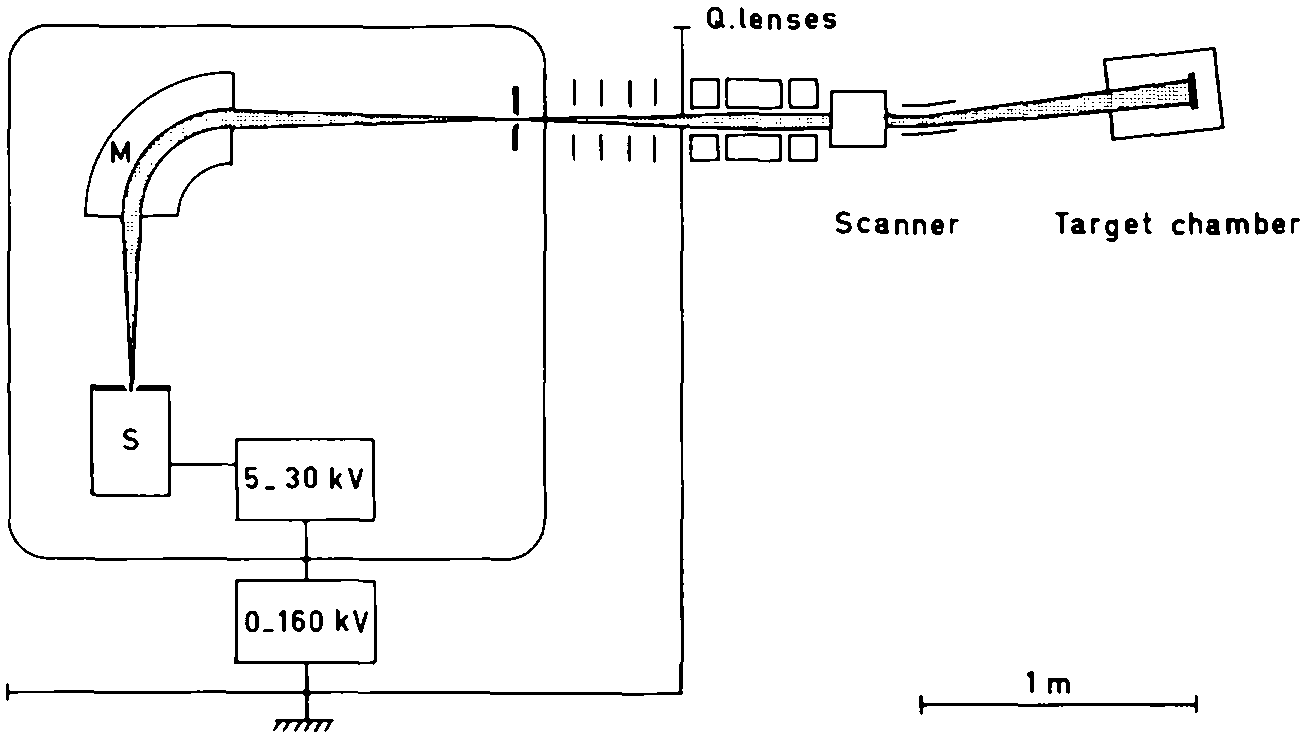
\includegraphics[width=\textwidth]{04_IPHI_Test/figures/fig000_IRMA01.png}
		\caption{}
		\label{}
	\end{subfigure}
	~
	\begin{subfigure}{0.5\textwidth}
		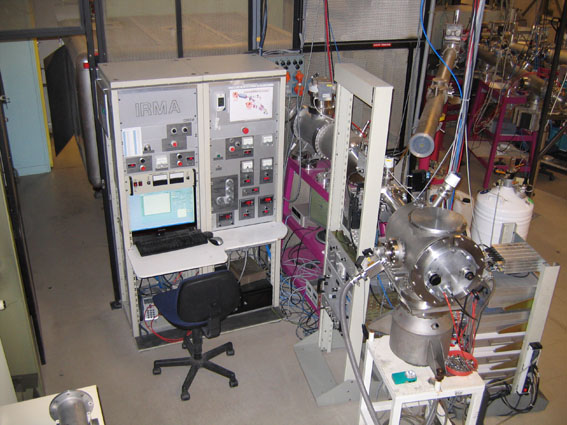
\includegraphics[width=\textwidth]{04_IPHI_Test/figures/fig000_IRMA02.jpg}
		\caption{}
		\label{}
	\end{subfigure}
	\caption[IRMA installation]{IRMA installation}
	\label{chap4:IRMA_facility}
\end{figure}


  \subsection{Test setup [C]}

  The test bench consists of a mechanical support on which is mounted the detector system. The current range at IRMA is important (from hundred $\mathrm{pA}$ to $\mathrm{\mu A}$) compared to the expected ionization current per ESS pulse (few $\mathrm{fA}$). The average current have been reduced by the following solutions. The beam was scanned in both directions at $80 \,\mathrm{Hz}$ and $400\,\mathrm{Hz}$ on a perpendicular stopping plate. A hole is drilled at the center of the plate, reducing the current by a factor of $12723$. At the end, the number of incident particles is around hundred thousand (hundred $\mathrm{fA}$) per IRMA “pulse”. A simple Faraday cup measures the current after reduction. The entire setup is visible in the Fig. \ref{chap4:IRMA_setup}.

  \begin{figure}[!ht]
	\begin{subfigure}[t]{0.5\textwidth}
		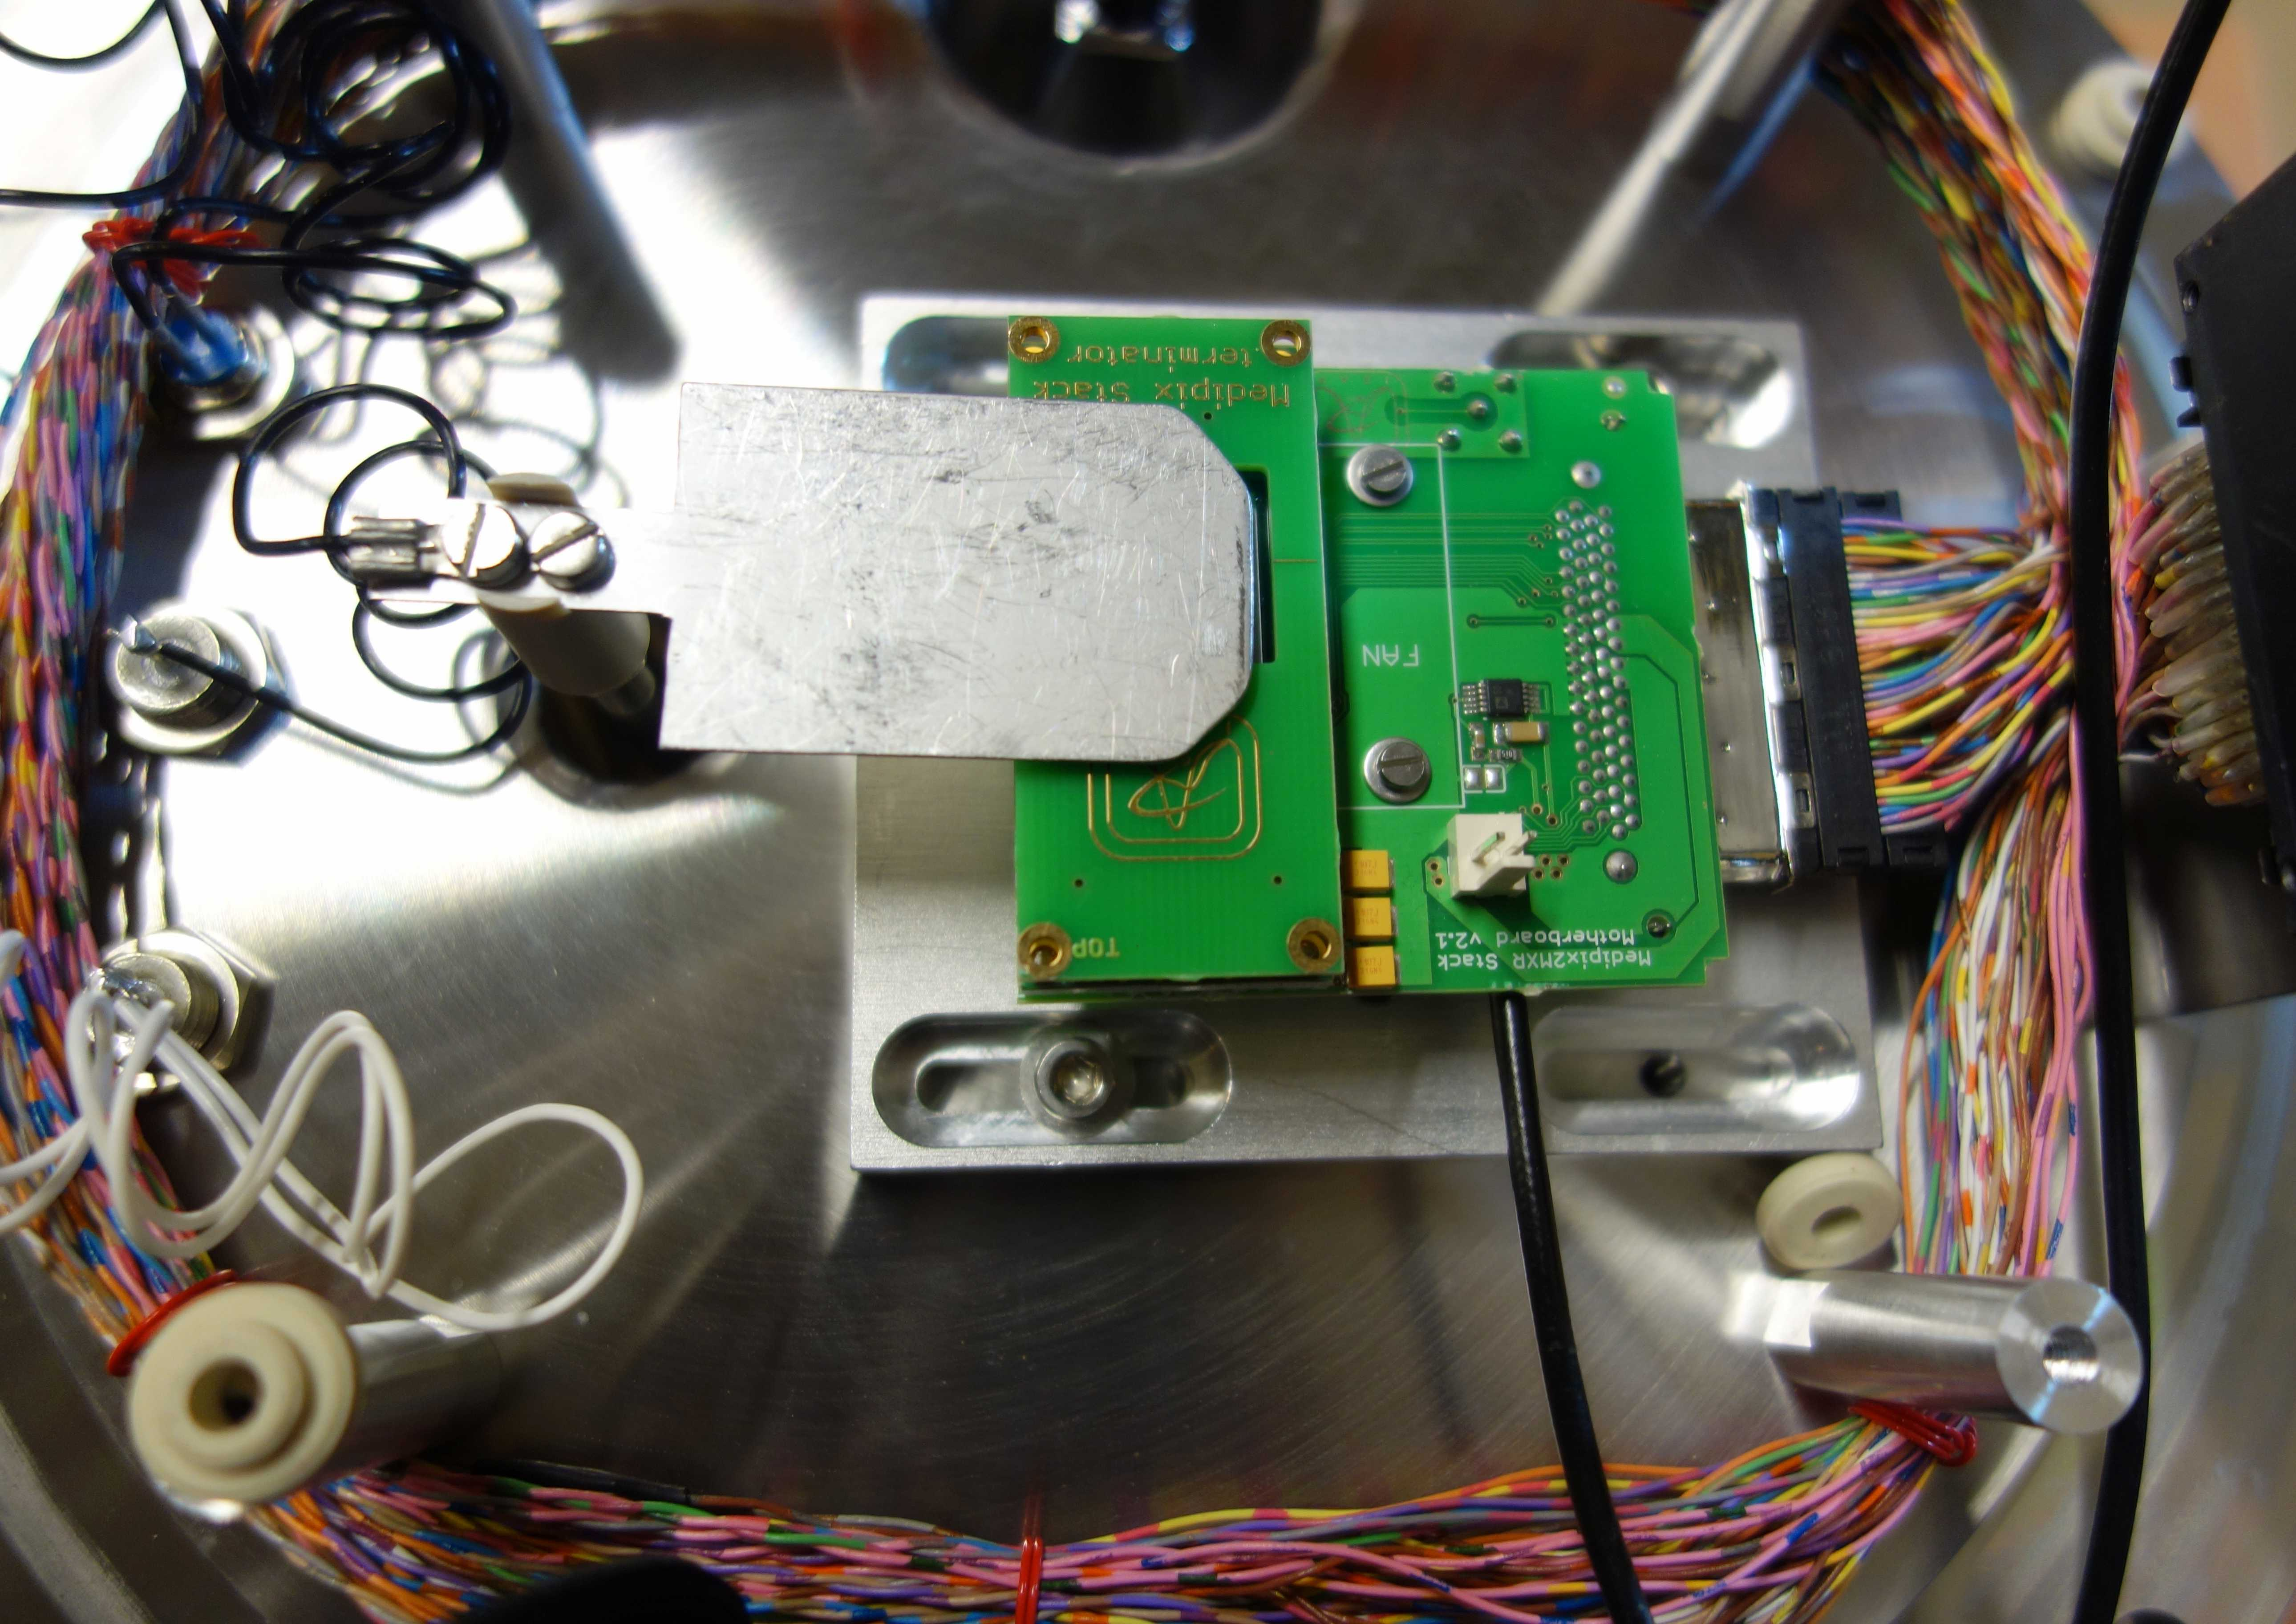
\includegraphics[width=\textwidth]{04_IPHI_Test/figures/fig000_IRMA_setup01}
		\caption{The TimePix chip is just behind the Faraday cup.}
		\label{}
	\end{subfigure}
	~
	\begin{subfigure}[t]{0.5\textwidth}
		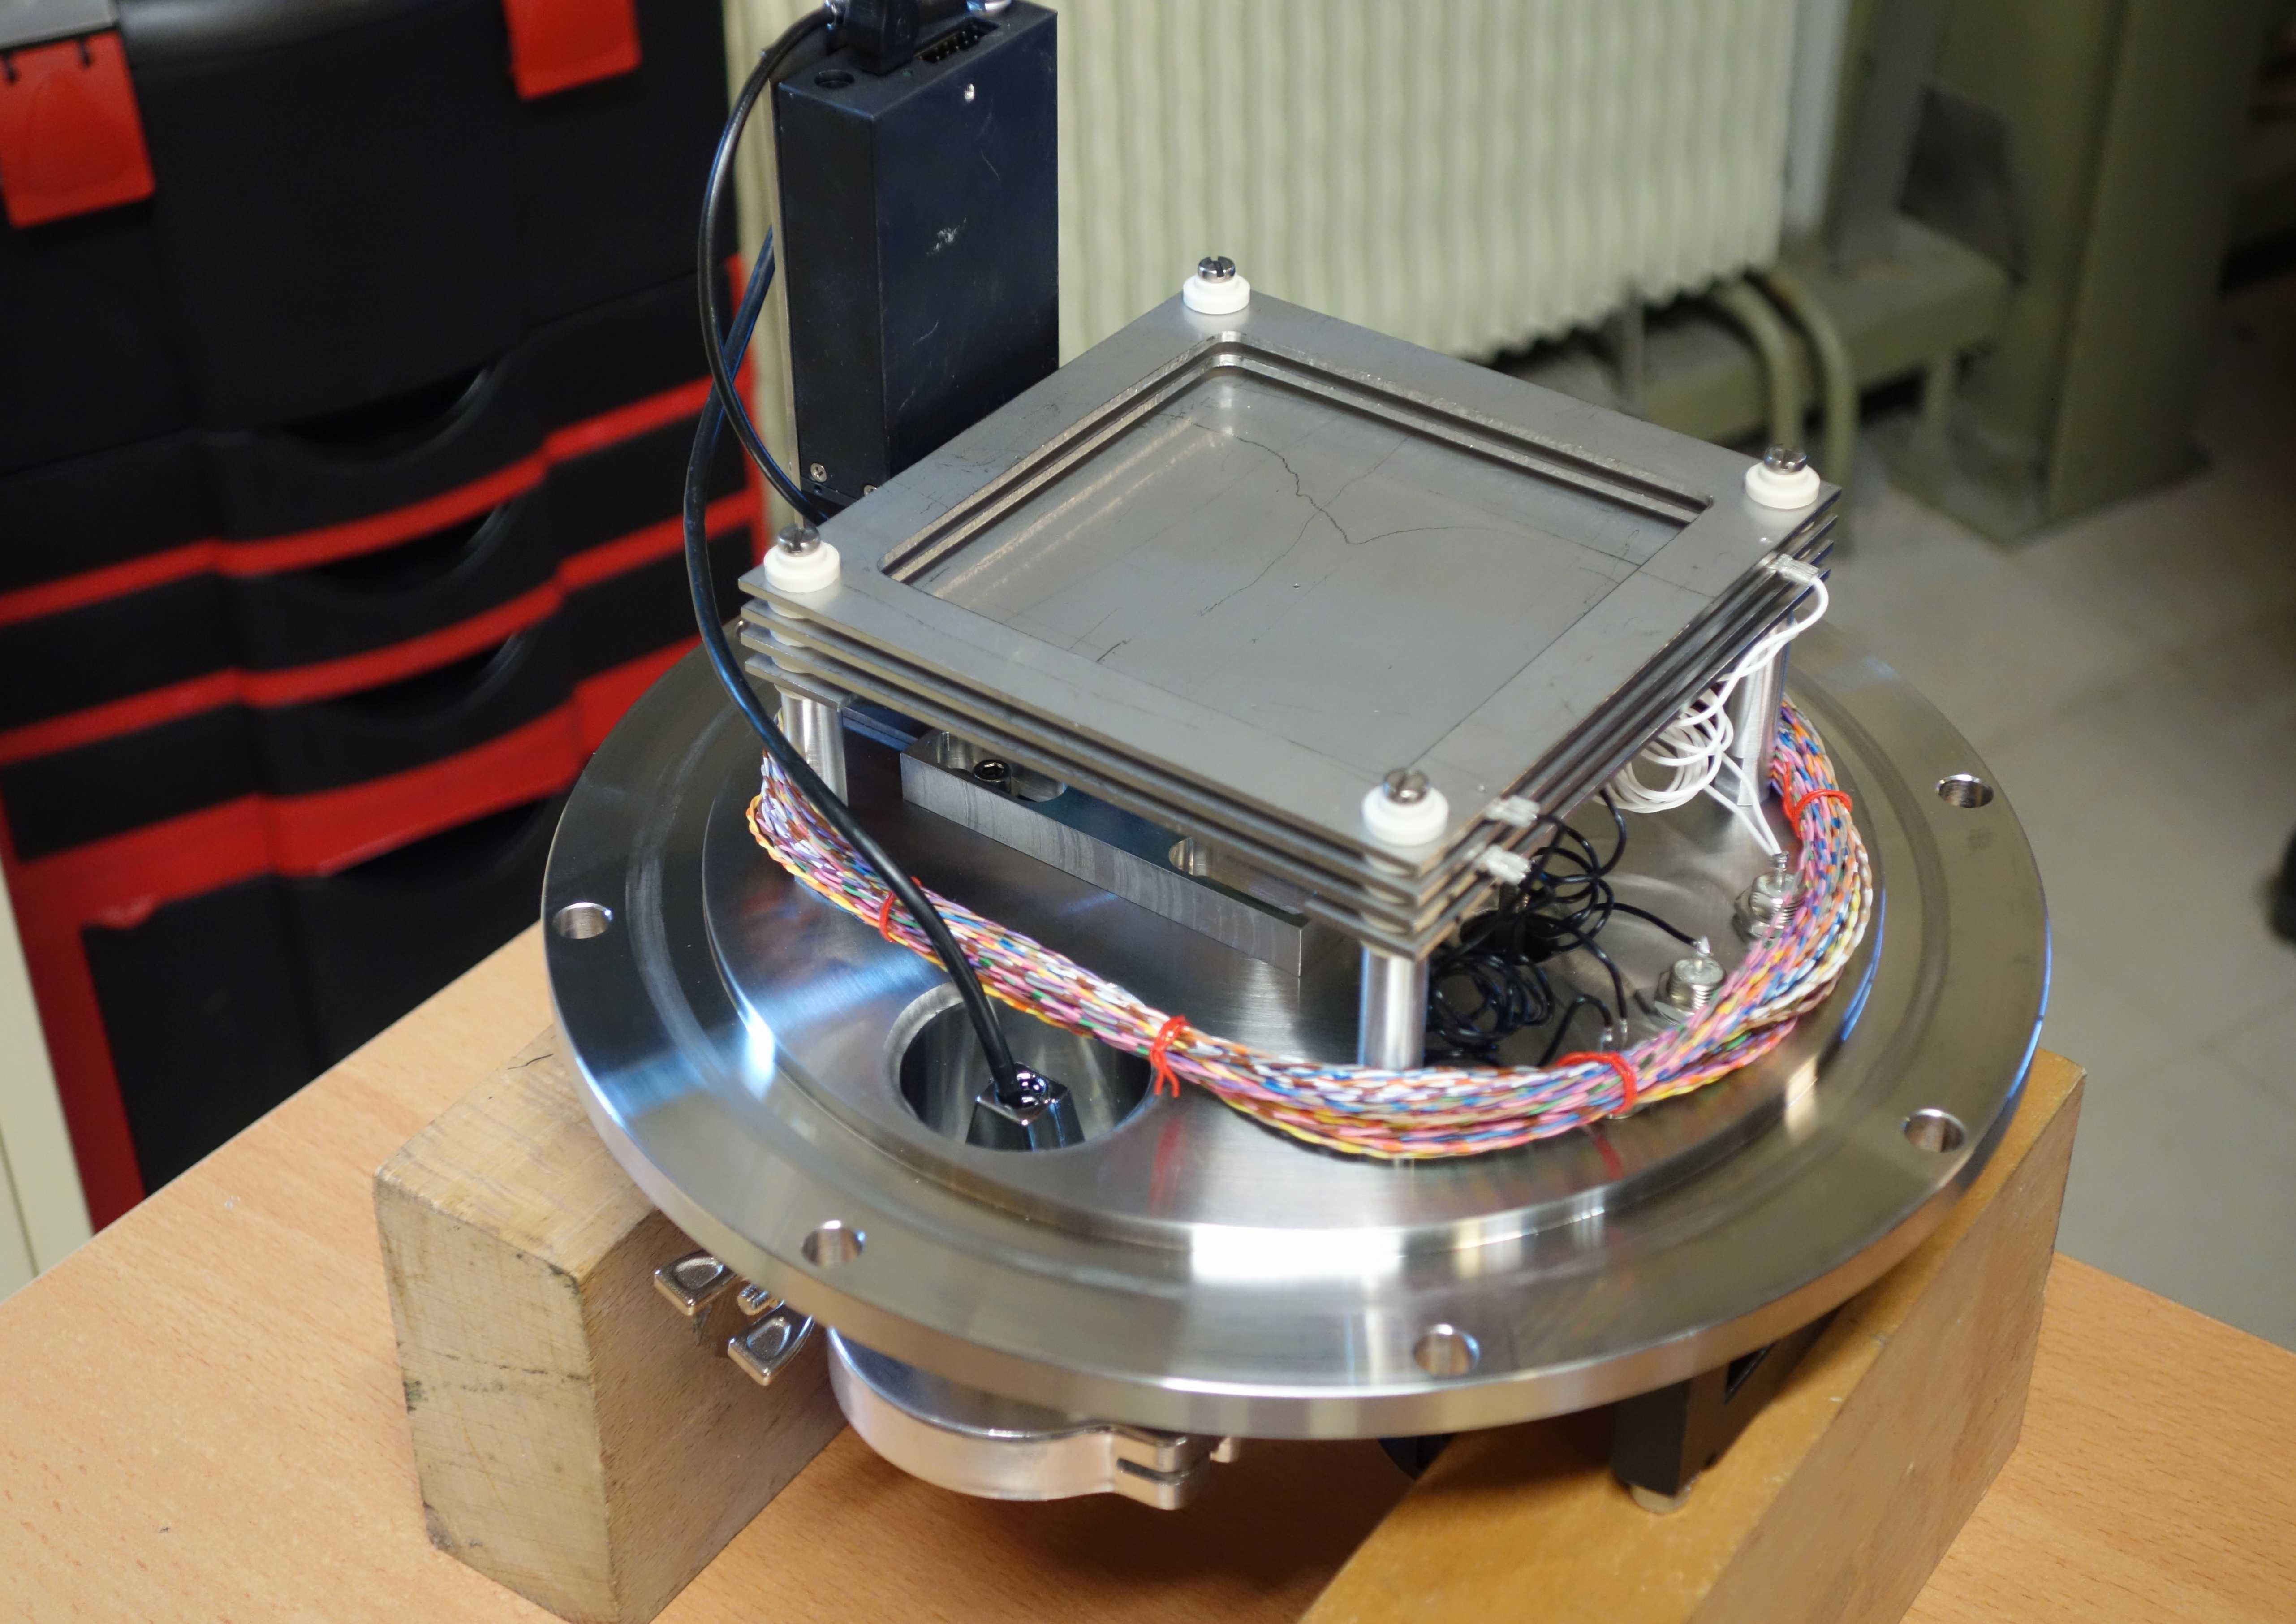
\includegraphics[width=\textwidth]{04_IPHI_Test/figures/fig000_IRMA_setup02}
		\caption{A plate with a drilled hole reduced the incoming current. The beam is scanned on the plate.}
		\label{}
	\end{subfigure}
	\caption[IRMA setup]{IRMA setup. A dedicated test bench has been developed for testing the TimePix chips.}
	\label{chap4:IRMA_setup}
\end{figure}


  The detector tested at IRMA is a silicon pixelated matrix ($256 \times 256$ with a pixel size $56\,\mathrm{\mu m}$) on top of a TimePix chip. The matrix is ​​very specific since the metallization layer has been replaced by a heavily doped layer allowing the polarization of the detector. The TimePix measures either the Time over Threshold (ToT) or the Time of Arrival (ToA). ToT is the total time during which the signal generated by the incident particle is above a threshold set by the user. This value is therefore proportional to the energy deposited by the particles in the pixels. The ToA gives the time difference of an incident particle with respect to a reference time.

  In fact, we didn't not directly use TimePix, but a complete solution \cite{Kraus2011,advacam2019} integrating a reading electronics controllable by PC. The software allows to configure the TimePix and acquire images with the value of ToT or ToA for each pixel.

  \subsection{Results and limitations [C]}

  The test performed at IRMA concerns the determination of the detection limit with the lightest possible ions i.e. $H_{2}^{+}$. The images at two energies and integrated signal for a full scan are shown in Fig. \ref{chap4:IRMA_Si}. For $15\,\mathrm{keV}$ ions the detection seems to work correctly, but the signal vanishes for ions with an energy of $12\,\mathrm{keV}$ or less. The limit of detection is therefore between these two values, and is very close to the energy that ions can reach in the IPMs. The residual gas at ESS is mainly a compound of ions heavier than $H_{2}^{+}$. These heavy ions will not be detected by the readout, reducing the already low signal of the IPM.

  \begin{figure}[!ht]
	\begin{subfigure}{0.25\textwidth}
		\includesvg[width=\textwidth]{04_IPHI_Test/figures/fig000_IRMA_15keV}
		\caption{ToT image at $15\,\mathrm{keV}$}
		\label{}
	\end{subfigure}
	~
	\begin{subfigure}{0.25\textwidth}
		\includesvg[width=\textwidth]{04_IPHI_Test/figures/fig000_IRMA_12keV}
		\caption{ToT image at $12\,\mathrm{keV}$}
		\label{}
  \end{subfigure}
  ~
  \begin{subfigure}{0.5\textwidth}
		\includesvg[width=\textwidth]{04_IPHI_Test/figures/fig000_IRMA_sweep}
		\caption{Total signal on the sensor with respect to the ion energies.}
		\label{}
  \end{subfigure}
	\caption[Main results from IRMA tests with $H_{2}^{+}$ ions]{Main results from IRMA tests with $H_{2}^{+}$ ions.}
	\label{chap4:IRMA_Si}
\end{figure}

  \begin{wrapfigure}{r}{0.4\textwidth}
  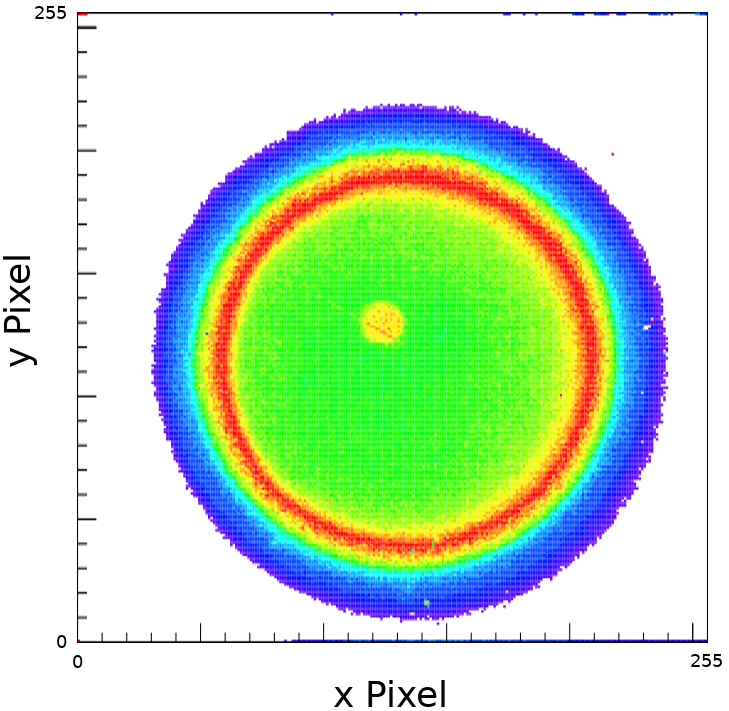
\includegraphics[width=0.4\textwidth]{04_IPHI_Test/figures/fig000_IRMA_damage2}
	\caption[The gain has changed after the irradiation]{The gain has changed after the irradiation.}
	\label{chap4:IRMA_damage}
\end{wrapfigure}

  Few days after the test, the integrity of the sensor has been test by illuminating it with an UV-VIS LED (peak emission at 365 nm). It emphasizes a small zone of the matrix, visible on Fig. \ref{chap4:IRMA_damage}, corresponding to the IRMA  beam position irradiation. Clearly the sensor was damaged, but unfortunately we can't give an accurate estimation of the deposited dose. Note that the gain has increased in the irradiated region.
  % A zone in the matrix and it is visible in Fig. \ref{chap4:IRMA_damage}.
  %  This zone is exactly in the same place as the one bombarded by the ions. The sensor has been probably deteriorated by the high current of IRMA. Unfortunately it is not possible to accurately estimate the number of ions that have been sent to the sensor and the nature of the damage is unknown. 

  Finally, we decided to give up with this technique for the signal weakness, not compliant with IPMs working in the mandatory  ion mode, and for the damages induces by ions as previously seen. The development cost of a silicon solution is not worth considering the possible risks of non-detection.
  In our quest for feasibility demonstration, we faced with this tool to several issues:
  \begin{itemize}
    \item No trigger, imposing to take long data run for avoiding to miss the beam interaction with the siicon detector.
    \item Beam scanning, despite calculations the beam sweeping of the detector varies time to time explaining partly our lack of knowledge for evaluating the dose.
    \item One day of data taking, with a total ignorance of IRMA as well as this kind of facility.
  \end{itemize}

  We hope to redo test for fully determining the detection limit of this method with ions and investigate more on the ion damaging.
  Since our test, TimePix3 has completely replaced its ancestor. This new version provides the ability to measure at a same time the ToT and ToA, with a higher timing resolution and an efficient data protocol. As well, the reading electronics has been improved allowing advanced triggering option of the chip.

  % We decided to not go further with silicon detectors for all the previous reasons. The cost of development of a silicon solution is not worth considering the possible risks of non detection. We would like to remain that the experiment has been done to quickly check the feasibility and it suffers from several limitations. Firstly the detector was not triggered, during short acquisitions pulse only very few data were taken in coincidence with the beam, therefore long acquisitions have been favored reducing the uncertainty only on the first and last pulse. The second uncertainty comes from the beam scanning. We noticed that, sometimes, the beam could pass through the hole more than once for a same scanning cycle. This means that the number of charge is collected by the TimePix is more than expected for an acquisition.


  \section{IPM design overview [C]}
  \subsection{IPM [C]}
  \begin{wrapfigure}{r}{0.5\textwidth}
  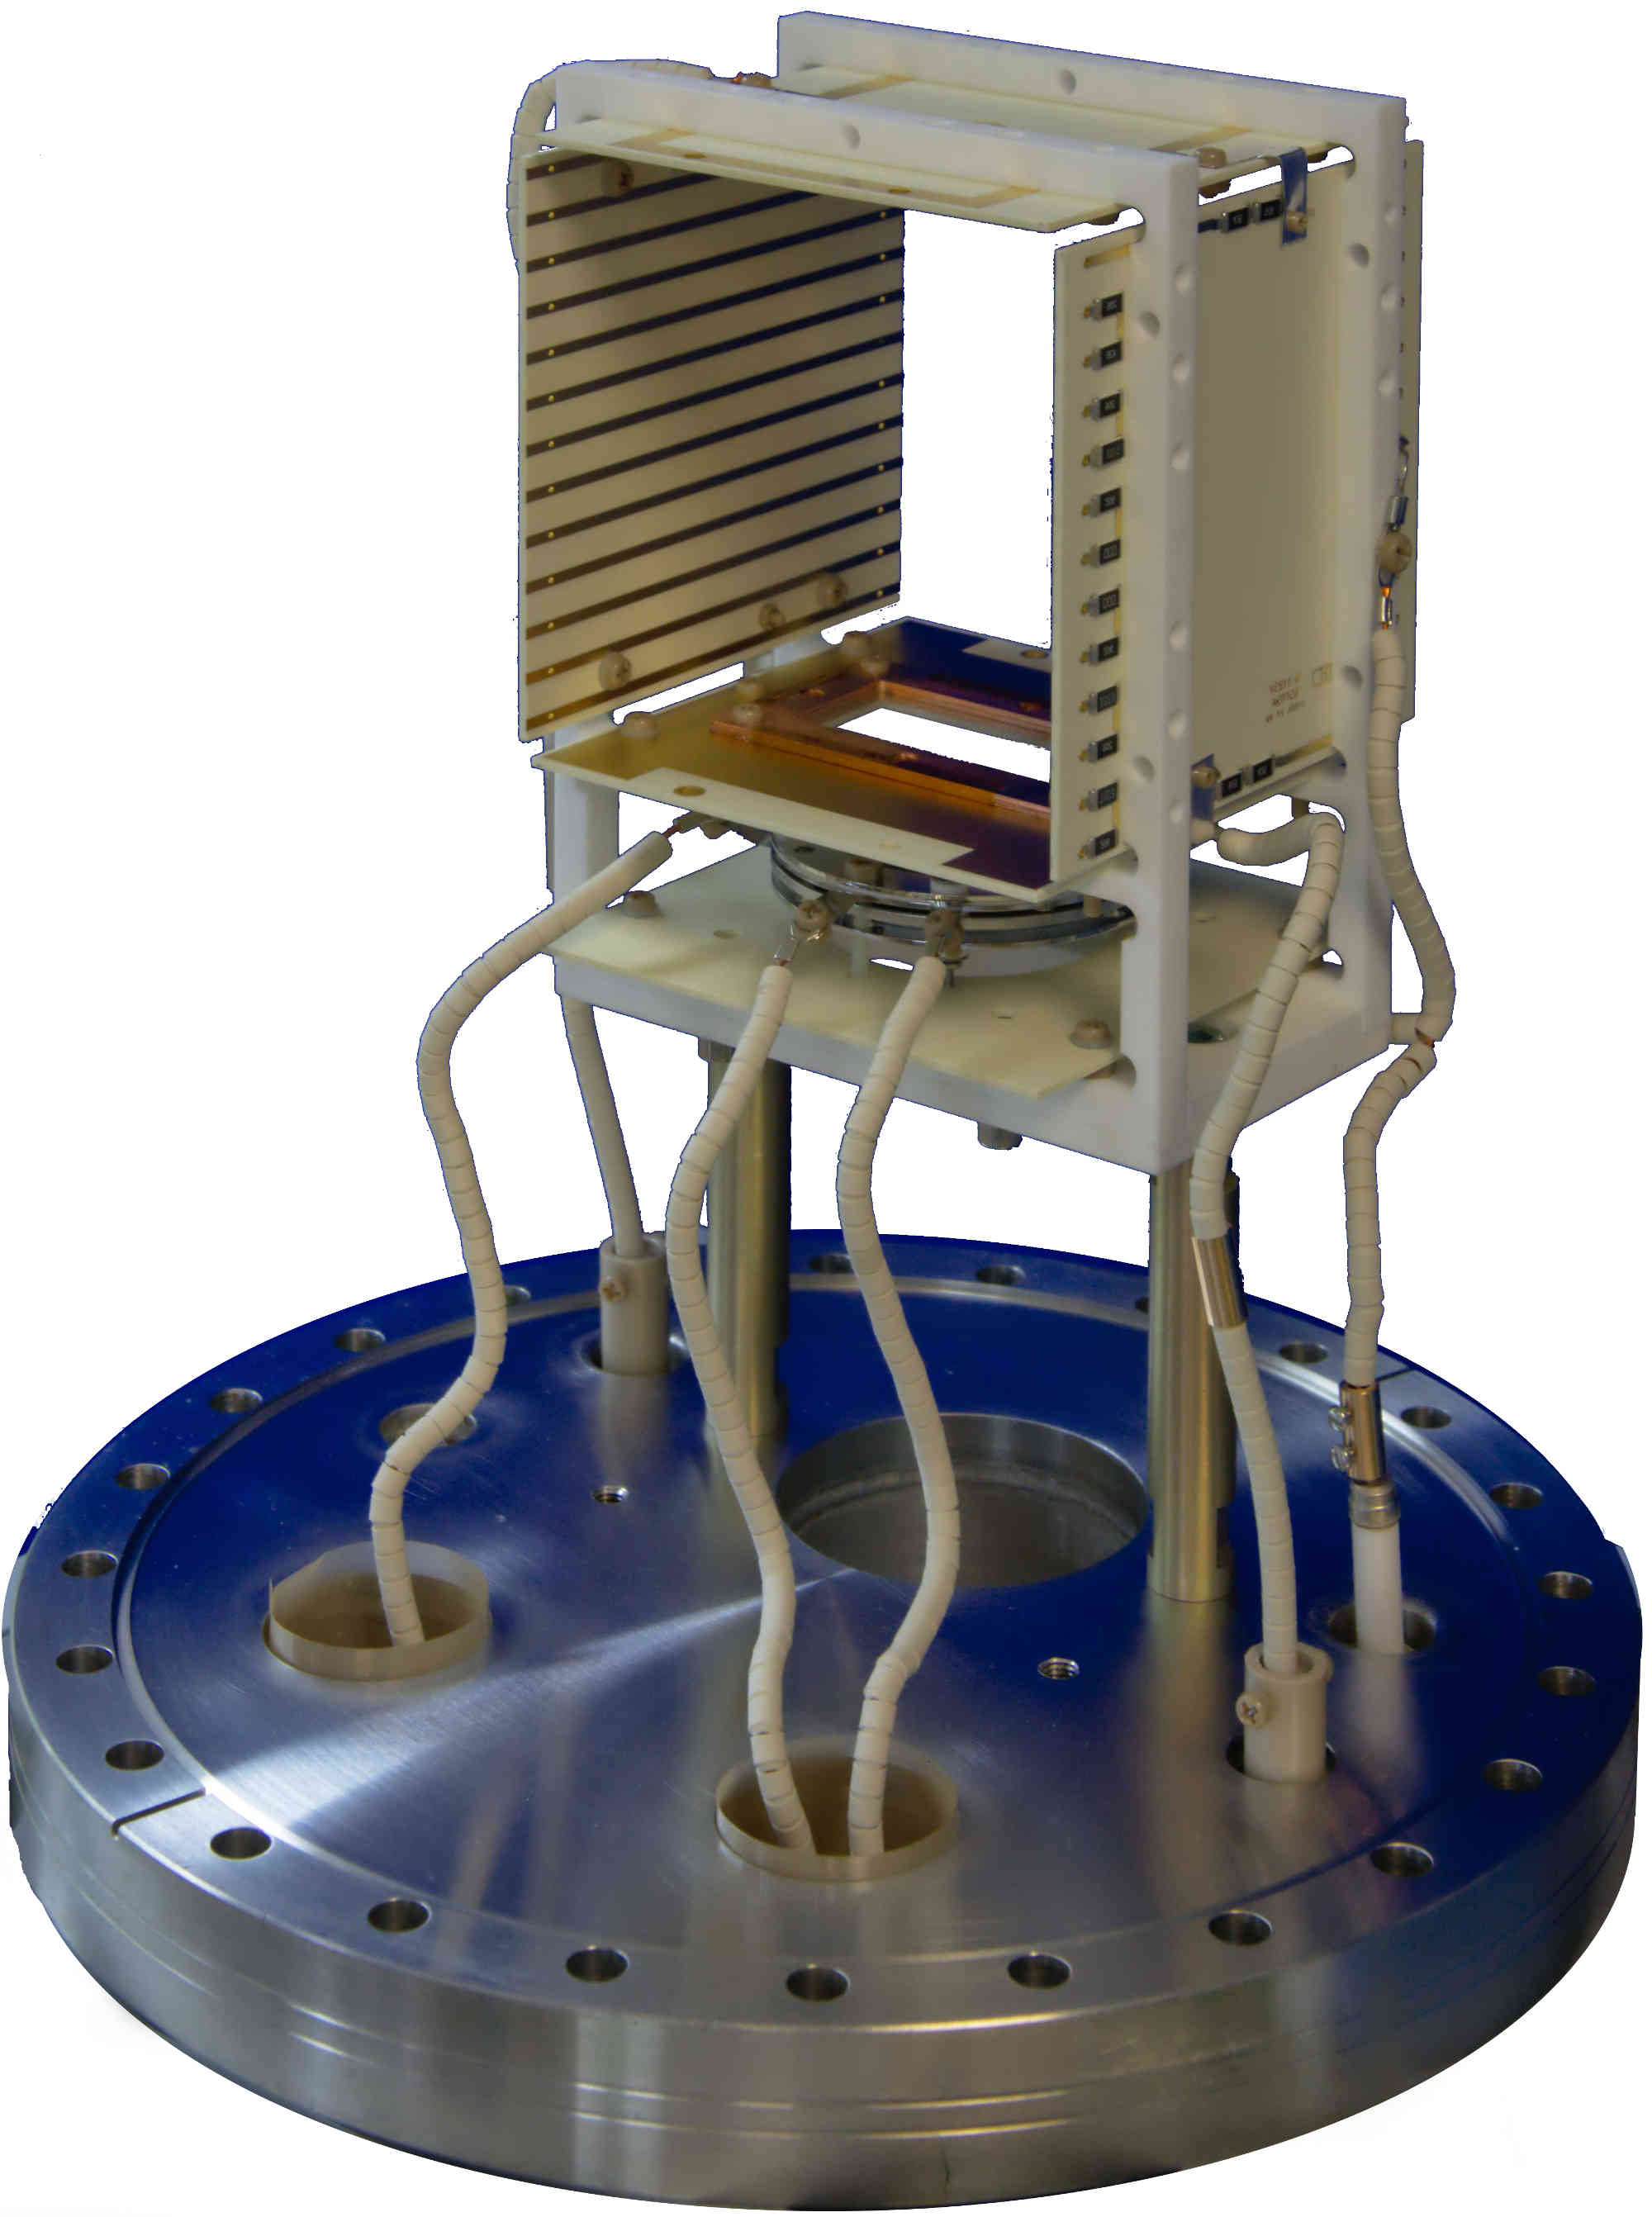
\includegraphics[width=0.5\textwidth]{04_IPHI_Test/figures/fig000_IPM_photo}
	\caption[]{}
	\label{chap4:IRMA_damage}
\end{wrapfigure}

  The IPM consists of five PCB plates: two for the electrodes, two for the field correctors and one for supporting the readout. The two electrode plates face each other, as well as the correction plates. The eletrode closest to the readout is grooved in its center with a conductive grid fixed on it, for insuring the electric field uniformity (see explanations on the previous chapter). The top electrode has a $5.5\,\mathrm{mm}$ radius circular hole in its center to let passing the light from a calibration source. The field correctors were engraved directly on the inner PCB face and resistors are welded on the outer side. SMD resistor type $2512$ ($1\,\mathrm{\%}$ precision, $3000\,\mathrm{V}$ max) are used.

  All PCB boards are firmly encapsulated in two frames made of insulating material. Two materials have been used: PEEK and MACOR. MACOR is a machinable ceramic that provides very high electrical insulation (more than $50\,\mathrm{kV/mm}$ DC),  good thermal conduction and withstands high temperatures ($800\,\textdegree{}C$). It is also compatible with vacuum despite its porous appearance. Even if it has very interesting mechanical properties, it must be handled with care \footnote{The author personally attest to this after handling one of the MACOR frames.}. PEEK (Polyether Ether Ketone) is a plastic polymer used in aggressive chemical environments. It is both an electrical (around $16\,\mathrm{kV/mm}$) and thermal insulator. It does not tolerate temperatures above $50\,\textdegree{}C$. PEEK can be used under vacuum, but its performance is much lower than MACOR. On the other hand, it is cheap and easy to handle.

  The two frames are screwed to a MACOR support fixed on the flange via two stainless steel rods. The ceramic support ensures a perfect insulation of the IPM with the vacuum chamber. The IPMs has been designed so that the cage is completely independent of the readout used. For IPMs using strips, it is also possible to rotate the IPM by $90\,\textdegree{}$ to change the direction of the measurement. The connections to the different high voltages are wired with bare copper  protected by ceramic beads. Vacuum feedthroughs are COTS components that can support voltages up to $30\,\mathrm{kV}$.

  \subsection{MCP [C]}
  A total of four MCPs has been bought from two different suppliers: Hamamatsu and Photonis. A simple single stage MCP and a single stage MCP coupled with a phosphorus screen. The simples MCPs will be used with the strips IPMs if the signal becomes too low.

  The MCP and phosphorus assemblies are key components of the optical and two different phosphorus screens has:
  \begin{itemize}
    \item P43 is a very luminescent material but has a strong remanence
    \item P46 that has a fast decay time but lower yield.
  \end{itemize}
  Since intra-pulse acquisition is not a requirement for ESS both screen may be considered.

  The characteristics of each MCP (and phosphorus screen) are given in the Table \ref{chap4:MCP_Phosphor}.
  \begin{table}[ht]
  \centering
  \caption[The main characteristics of MCPs used during the beam tests]{The main characteristics of MCPs used during the beam tests. MCPs from Hamamatsu has the same characteristics except that one has a phosphorus screen as readout.}
  \label{chap4:MCP_Phosphor}
  \begin{tabular}{llll}
    \toprule
                     & Hamamatsu         & Photonis 1                  & Photonis 2                  \\
    \midrule
    Active radius    & $40\,\mathrm{mm}$           & $40\,\mathrm{mm}$           & $40\,\mathrm{mm}$           \\
    Channel diameter & $12\,\mathrm{\mu m}$        & $10\,\mathrm{\mu m}$        & $25\,\mathrm{\mu m}$        \\
    Channel pitch    & $15\,\mathrm{\mu m}$        & $12\,\mathrm{\mu m}$        & $32\,\mathrm{\mu m}$        \\
    OAR              & $60\,\mathrm{\%}$           & $55\,\mathrm{\%}$           & $45\,\mathrm{\%}$           \\
    Bias angles      & $8\,\mathrm{\textdegree{}}$ & $8\,\mathrm{\textdegree{}}$ & $8\,\mathrm{\textdegree{}}$ \\
    \midrule
    Screen type      & $P43$                  & $P46$                       & -                           \\
                     & $Gd_{2}O_{2}S:Tb$           & $Y_{3}Al_{5}O_{12}:Ce$      &                             \\
    Gain relative    & $1$                      & $0.3$                       & -                           \\
    Wavelength       & $545\,\mathrm{nm}$      & $530\,\mathrm{nm}$          & -                           \\
    Decay time range & $\mathrm{ms}$           & $\mathrm{\mu s}$            & -                           \\
    \bottomrule
  \end{tabular}
\end{table}

  \subsection{Camera [C]}
  A vision system is necessary for recording light from the phosphorus screen.
  A camera with a lens should be sufficient in our case.

  % Sensor
  The sensor is the core component of a camera, so it is better to choose it first, on the basis of the requirements.
  For our application high resolution is not mandatory, so pixels could be relatively big in order to increase light collection and dynamic range.
  Sony IMX249 fits well with these prerequisites. It is a consumer CMOS sensor with relatively big pixels and low noise.
  Its EMVA characteristics are summarized in the Table \ref{tab:IMX249} \cite{emva2010}.
  \begin{table}[!h]
  \centering
  \caption{Main features of the Sony IMX249 sensor}
  \label{tab:IMX249}
  \begin{tabular}{ll}
    \toprule
    Resolution           & 1936 (H) * 1216 (V)  \\
    Pixel size           & 5.86 $\mu m$         \\
    Sensor diagonal size & 13.4 mm (Type 1/1.2) \\
    Well capacity        & 32000 e-             \\
    Dynamic Range        & 70 dB                \\
    QE at 525 nm         & 70 \%                \\
    Electrons noise      & 6.8 $e^{-}$          \\
    ADC                  & 8, 10 or 12 bits     \\
    Max framerate        & 30 fps               \\
    \bottomrule
  \end{tabular}
\end{table}

  % Camera
  AlliedVision, Basler and FLIR propose several cameras based on the IMX249 sensor with different interfaces, features, form factors, prices and availability.
  We restricted our choice to GigE cameras since they allow long cable length and Power over Ethernet (PoE) which are quite useful features for an accelerator experiment.
  At the end we chose the FLIR Blackfly-PGE-23S6M-C \cite{blackfly2019}.

  % Lens
  The last step is the choice of a correct lens for the camera.
  Unfortunately lens suppliers do not provide full characteristics of their lenses, hence only the thin lens approximation has been considered in our calculations. The distance from the back of the phosphorus screen to the external air-side of the viewport is $247\,\mathrm{mm}$. The active area radius of our MCPs is around $25\,\mathrm{mm}$, while the sensor side measures $11.34\,\mathrm{mm}$. The required magnification therefore amounts to $0.2268$ at least.
  Table \ref{tab:lens_magnification} shows magnification factors for several focal lengths. So, a focal length of 50 mm fits very well with our configuration.
  \begin{table}[!h]
  \centering
  \caption[Magnification for several common focal lengths]{Magnification for several common focal lengths, at a working distance of $247\,\mathrm{mm}$.}
  \label{tab:lens_magnification}
  \begin{tabularx}{1\textwidth}{lllllllll}
    \toprule
    Focal length ($\mathrm{mm}$) & $5$    & $15$    & $28$    & $35$    & $50$    & $75$    & $100$  & $150$   \\
    Magnification     & $0.02$ & $0.069$ & $0.127$ & $0.165$ & $0.255$ & $0.436$ & $0.68$ & $1.546$ \\
    \bottomrule
  \end{tabularx}
\end{table}

  Lenses with $50\,\mathrm{mm}$ focal length are rather standard and commercially available at moderate cost. In addition these lenses have a large numerical aperture (or small F-number) so they provide a large photon capture efficiency.

  \subsection{Strips [C]}
  The strips were manufactured in the same way as the other PCBs presented above. Two strip configurations have been foreseen. The first one is the linear strips: the strips have the same width of $800\,\mathrm{\mu m}$ and an identical spacing of $920\,\mathrm{\mu m}$. A total of 32 strips were etched on the PCB, representing an active area of about $3\,\mathrm{cm}$. The second version is called Gaussian because the strips on the borders are wider than the ones in the center. The idea is that the strips on edges detect only few particles, so it is not necessary to have very thin strips since they will probably be in the noise. Therefore, the number of strips is reduced to $18$ with variable width from $0.8\,\mathrm{mm}$ to $9\,\mathrm{mm}$, leading to a total active area of $5\,\mathrm{cm}$. The table gives the values for the first $9$ gaussian strips, the $9$ remaining strip are the mirror of the first ones.

  \begin{table}[!ht]
  \centering
  \caption[Positions and sizes of the first half of gaussian strips]{Positions and sizes of the first half of gaussian strips.}
  \label{chap4:GaussianStrips}
  \begin{tabularx}{\linewidth}{lXXXXXXXXX}
    \toprule
    Strip    & 1     & 2    & 3    & 4    & 5    & 6    & 7    & 8    & 9    \\
    \midrule
    Size ($\mathrm{mm}$)    & 9     & 5    & 3    & 2    & 1.5  & 1    & 0.9  & 0.8  & 0.8  \\
    Position ($\mathrm{mm}$) & 20.52 & 13.4 & 8.28 & 6.66 & 4.79 & 3.42 & 2.35 & 1.38 & 0.46 \\
    \bottomrule
  \end{tabularx}
\end{table}
%   \centering
%   \setlength\tabcolsep{1.5pt}
%   \scalebox{0.8}{
%     \begin{tabular}{l| c |c | c } \hline \hline
%       STRIP NUMBER  \hspace*{1.5cm} & \hspace*{0.75cm} x\_min \hspace*{0.75cm} & \hspace*{0.75cm} x\_max \hspace*{0.75cm} & \hspace*{0.75cm} width \hspace*{0.75cm} \\
%       \hline \hline
%       1                             & -25.02                                   & -16.02                                   & 9                                       \\
%       2                             & -15.9                                    & -10.9                                    & 5                                       \\
%       3                             & -10.78                                   & -7.78                                    & 3                                       \\
%       4                             & -7.66                                    & -5.66                                    & 2                                       \\
%       5                             & -5.54                                    & -4.04                                    & 1.5                                     \\
%       6                             & -3.92                                    & -2.92                                    & 1                                       \\
%       7                             & -2.80                                    & -1.90                                    & 0.9                                     \\
%       8                             & -1.78                                    & -0.98                                    & 0.8                                     \\
%       9                             & -0.86                                    & -0.06                                    & 0.8                                     \\
%       10                            & 0.06                                     & 0.86                                     & 0.8                                     \\
%       11                            & 0.98                                     & 1.78                                     & 0.8                                     \\
%       12                            & 1.9                                      & 2.8                                      & 0.9                                     \\
%       13                            & 2.92                                     & 3.92                                     & 1                                       \\
%       14                            & 4.04                                     & 5.54                                     & 1.5                                     \\
%       15                            & 5.66                                     & 7.66                                     & 2                                       \\
%       16                            & 7.78                                     & 10.78                                    & 3                                       \\
%       17                            & 10.9                                     & 15.9                                     & 5                                       \\
%       18                            & 16.02                                    & 25.02                                    & 9                                       \\
%       \hline \hline
%     \end{tabular}}
%   \caption{Gaussian detector geometry.}
%   \label{tab:det2}
% \end{table}

  \subsection{CARAMEL board and FASTER system [C]}

  The strips are read by the CARAMEL card \cite{caramel2013} from the FASTER system. FASTER is a versatile  acquisition platform developed by LCP at Caen \cite{faster2013}. CARAMEL is an electrometer VITA-57 card based on two DDC316 chips from Texas Instrument \cite{ddc316}. Each chip integrates 16 acquisition channels connected to a dual integrator circuit allowing continuous measurement. The DDC316 chip covers integration times from $10\,\mathrm{\mu s}$ to $1\,\mathrm{ms}$ and three measurement ranges are available: $3\,\mathrm{pC}$, $6\,\mathrm{pC}$, $12\,\mathrm{pC}$. The DDC316 can read only positive charges, so an homemade current injector has been developed to add an offset allowing the measurement of negative charges.
  \begin{figure}[!ht]
	\begin{center}
		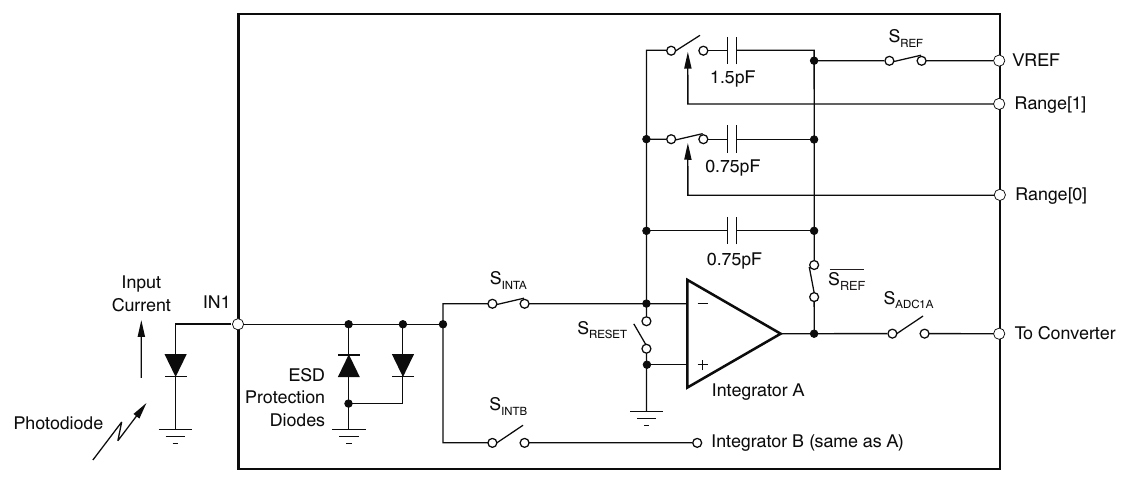
\includegraphics[width=\textwidth]{04_IPHI_Test/figures/fig000_DDC316}
	\end{center}
	\caption[]{}
	\label{chap4:DDC316}
\end{figure}


  Two CARAMEL boards can be plugged in a motherboard compatible with microTCA crates. All modules in a crate are controlled by a software that configures the entire system, runs acquisitions and visualizes \cite{rhb2012} the data online. The data can be saved in a binary format and a library allows to read them afterward.

  \section{High voltage power supplies [C]}
  An IPM requires high voltages to create the extraction field and to supply the MCP when it is used as readout. All power supplies come from iseg-HV \cite{iseg2019} and cover range from $0\,\mathrm{kV}$ to $30\,\mathrm{kV}$ with negative or positive polarities.

  MCPs allow complete floating configuration. This means that the readout can work at very high potential. We refer this configuration as symmetric since the MCP is at the opposite value of the extracting electrode, as explained in previous chapter. In this case the electric field is more uniform if no corrections are applied. However, it increases the number of high voltage power supplies and the design complexity (Fig. \ref{chap4:setup_asym}).
  Of course MCPs work also correctly at ground (Figure \ref{chap4:setup_asym}), we refer this set-up as asymmetric. The strips IPMs support only the asymmetric configuration and do not require more than one high voltage. During the two test campaigns we were able to work in both configuration.

  \begin{figure}[!ht]
  \begin{subfigure}[t]{0.5\textwidth}
    \centering
    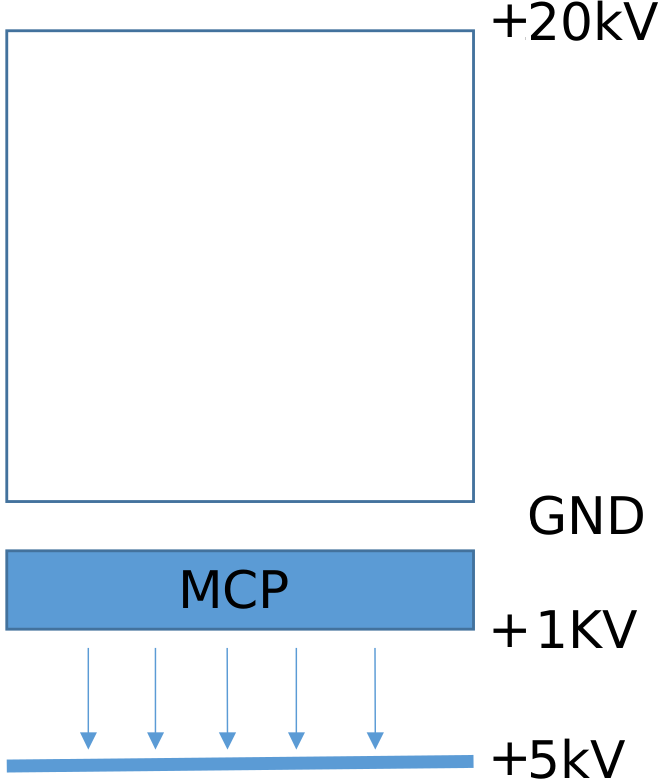
\includegraphics[width=0.7\textwidth]{04_IPHI_Test/figures/fig000_setup_hv_asym2}
    \caption{Asymmetric configuration.
    Readout is grounded while extracting electrode is at a certain potential.}
    \label{chap4:setup_hv_asym}
  \end{subfigure}
  ~
  \begin{subfigure}[t]{0.5\textwidth}
    \centering
    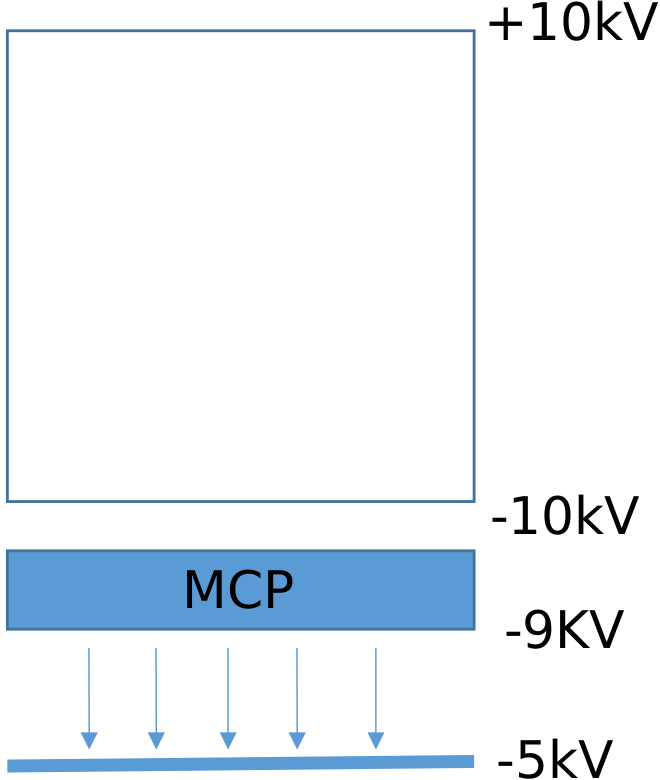
\includegraphics[width=0.7\textwidth]{04_IPHI_Test/figures/fig000_setup_hv_sym}
    \caption{Symmetric configuration. Readout and extracting electrode are at opposite potential.}
    \label{chap4:setup_hv_sym}
  \end{subfigure}
  \caption[Asymmetric or symmetric configuration]{Asymmetric or symmetric configuration, MCPs allow both.}
  \label{chap4:setup_hv}
\end{figure}


  \subsection{Control System [C]}
  The whole ESS Control System (CS) will rely on the EPICS (Experimental Physics and Industrial Control System) toolkit. The ESS CS team has specified its own EPICS standards to ensure the sustainability of the control system over the years. We will also test our IPMs at an accelerator whose control system is EPICS compatible. Therefore, EPICS has some importance to our project and we tried to use it as much as possible for our prototypes. In this section we will briefly describe EPICS and how we have integrated our test bench under such environment.

  EPICS provides a set of tools and protocols to facilitate the integration of control systems \cite{epics2019}. Originally developed for real-time systems, it now supports many platforms. EPICS has become an open source project in 2004, since many laboratories and collaborations have contributed to its development.
  One of the most important component of EPICS is the Channel Access (CA). In few words, it is a protocol that defines how the data are exchanged between clients and servers on a network. A server provides Processes Variables (PV) to clients. A PV is a useful data (for instance a current, a voltage or a temperature) associated with metadata (timestamp, units). A client can access and edit a PV value by knowing its name. In practice a server is often an hardware controlled by software, often called software Input / Output Controller (softIOC). A client is for instance an operator interface (OPI) which allows to view and modify the PV from one or more softIOCs.

  The whole system employed for the test bench is almost fully compatible with the version 3.16 of EPICS base. The PointGrey GigE cameras are well supported by the AreaDetector module \cite{ad2019}. A custom plugin, developed by ESS, performs a gaussian fit on the profile every image. Raw images are saved into HDF5 files \cite{hdf5}. This format allows to pack  various datasets together, for instance the raw IPM images with some beam information.
  Since all high voltage power supplies have their own SPCI Ethernet interface, thus a simple softIOC with StreamDevice\cite{streamdevice2019} was enough to control and monitor them.
  Three OPIs have been developed in order to control cameras, power supplies and a GEO BRICK controller\footnote{Motor to move scintillating screens vertically to intercept the beam or to be safely moved far from it.}. They run under the BOY module of the ESS Control System Studio version 4.5. An Archiver Appliance records and saves slow process variables from the power supplies, the vacuum systems and the accelerator \cite{archiver2019}.

  %%%%% controler le footnote à propos de Geobrick

  \begin{figure}[!ht]
	\begin{center}
		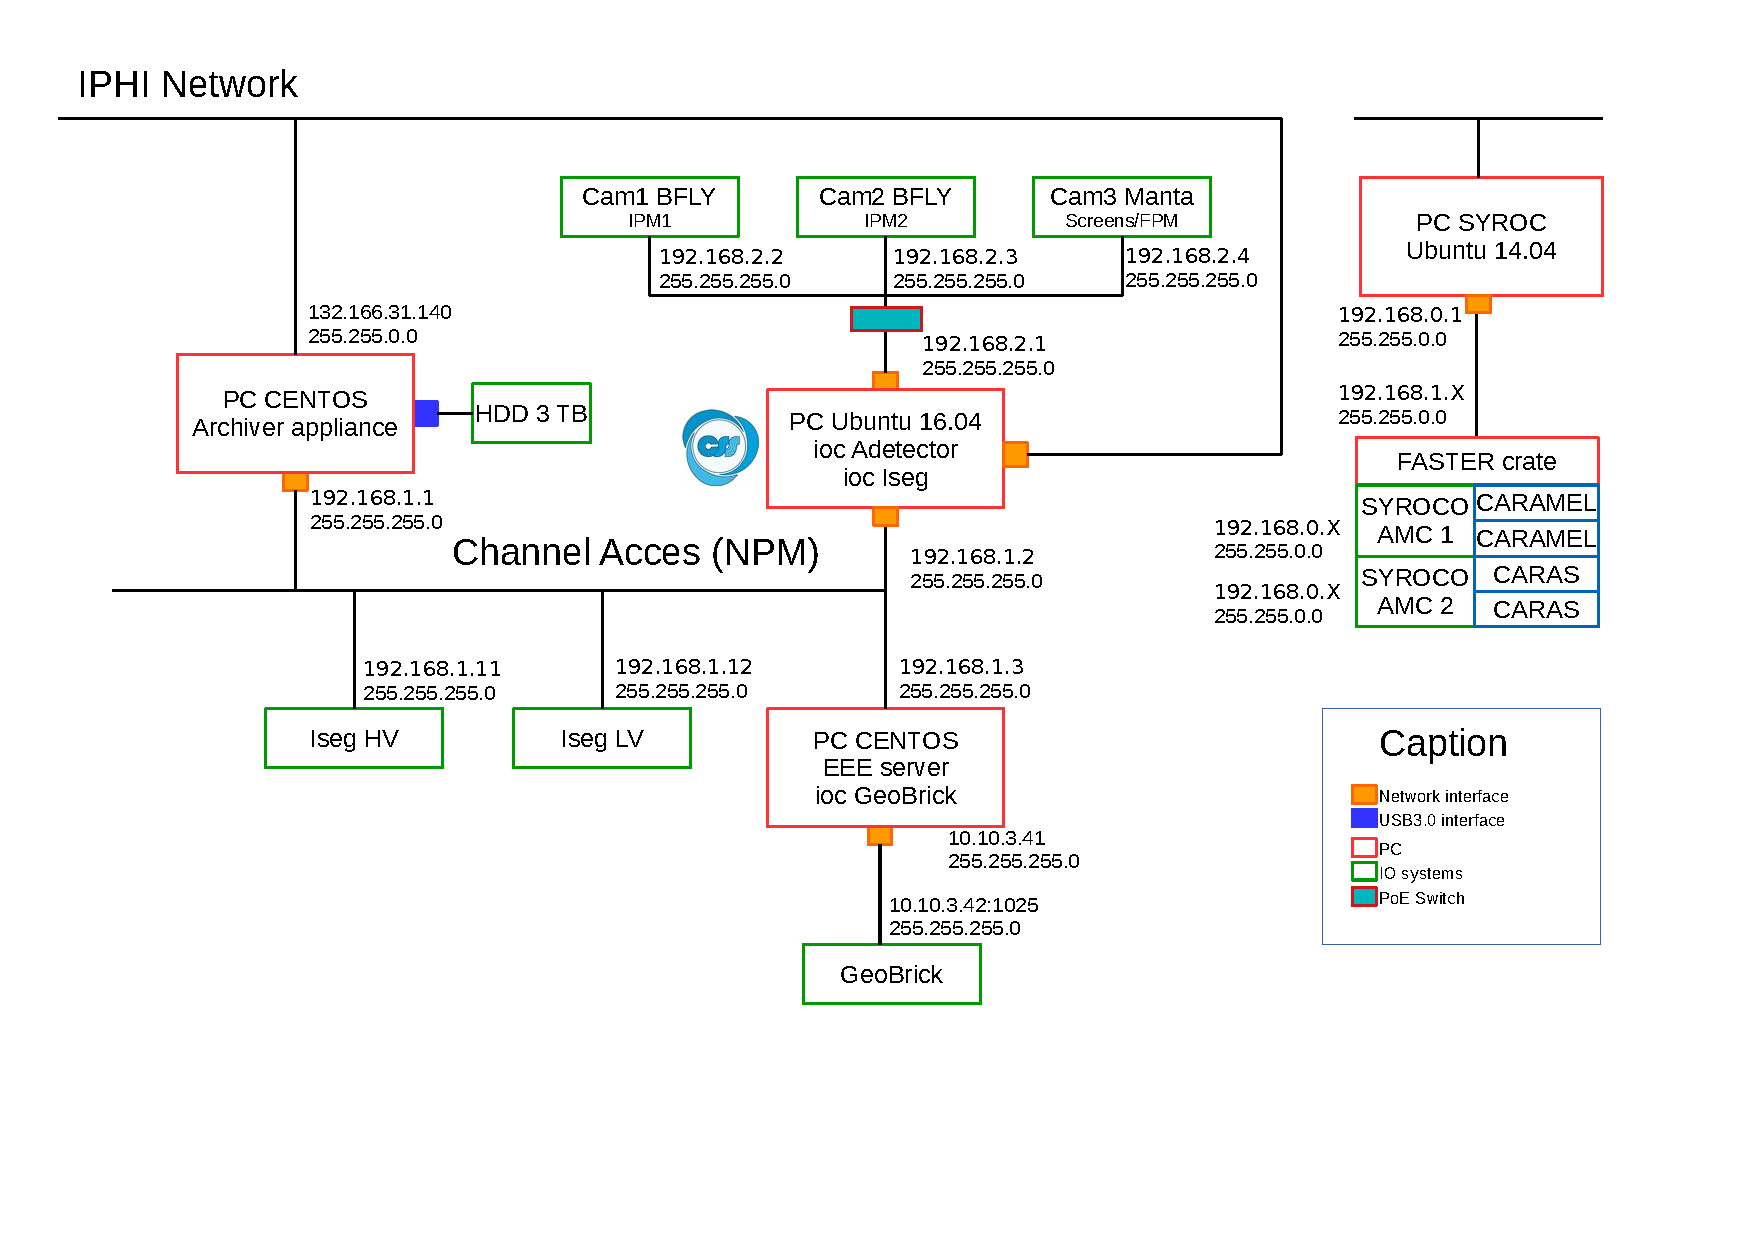
\includegraphics[width=\textwidth]{04_IPHI_Test/figures/fig000_EPICS_IPHI.pdf}
	\end{center}
	\caption[EPICS network setup during beam tests]{EPICS network setup during beam tests.}
	\label{chap4:EPICS_IPHI}
\end{figure}


  \subsection{Test bench [C]}
  A test bench has been also developed in order to test the prototypes. The bench can be split into two different independent parts.

  The first part (upstream) tries to mimic the ESS LWU chamber (scale 1) on which two IPMs can be inserted. The idea is to be close to the ESS conditions in term of high voltages and electrical fields. The second part (downstream) offers one more IPM slot and two viewports for reference measurements in order to compare with the IPM ones. Fig. \ref{chap4:Testbench} is a technical drawing of the test bench. One can see the resemblance of the upstream part with the LWU vessel previously shown in Fig. \ref{chap3:LWU_Cryo} and \ref{chap3:COMSOL_LWU}.


  The IPMs can be mounted independently in Y or X directions thanks to their design, thus it is even possible to measure the same transverse profile with all three IPMs.

  \begin{figure}[!ht]
	\begin{center}
		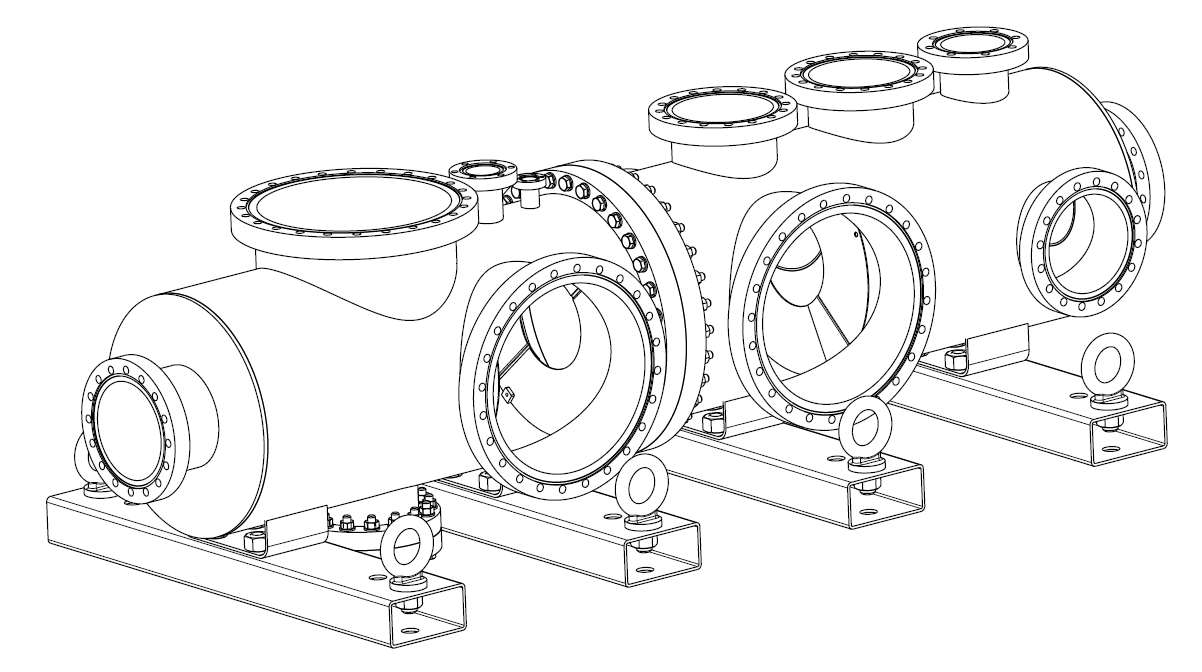
\includegraphics[width=\textwidth]{04_IPHI_Test/figures/fig000_Testbench.png}
	\end{center}
	\caption[IPM test bench]{IPM test bench. Left part is the LWU-like vessel
	while right part add more viewports for testing purposes.}
	\label{chap4:Testbench}
\end{figure}


  The test bench is pumped by 3 turbomolecular pumps with an average pumping speed of about $150\,\mathrm{L/s}$ at 3 different locations along the bench. The vessel can be baked using a heating system. The objective is to reach quickly the minimal vacuum level required to operate. Thus during the tests it is possible to modify the IPMs without sacrificing too much beam time. The whole system reaches a vacuum level of $1\cdot 10^{-7}\,\mathrm{mbar}$ in about ten hours (one night) after an intervention. An RGA and vacuum gauges monitor the vacuum level as close as possible to the IPMs.

  \subsection{Reference measurement [C]}
  A reference measurement is always a good practice when developing a detector. First, it may help to diagnostic possible issues on the prototypes. Then, it allows a complete comparison with the prototypes, and gives more confidence on the measurement. Therefore, two methods have been foreseen and implemented for this purpose.

  The first method uses scintillator screens, which is interceptive. The screens are mounted on a racket that can be inserted into the beam using a translator controlled remotely through a GEO BRICK controller. Three scintillator screens have been kindly provided by our colleagues at Saclay. Table \ref{chap4:tab_ecran} sums up the main characteristics of each screen.
  % and Fig \ref{chap4:fig_ecran} shows the three screens on a support.

  \begin{table}[ht]
	\centering
	\caption[]{Properties common semiconductors used as radiation detector.}
	\label{chap3:semiconductor}
	\begin{tabular}{llll}
    \toprule
    Property & $\mathrm{Prelude}420$ $(Lu^{1.8}Y.^{2}SiO^{5}:Ce)$ & $\mathrm{YAG:Ce}$ & $\mathrm{CdTeZn}$ \\
    \midrule
    Density &  &  &  \\
    Light yield &  &  &  \\
    Typical wavelength &  & & \\
		\bottomrule
	\end{tabular}
\end{table}

  The second system foreseen is a Fluorescence Profile Monitor (FPM). This system is developed by our ESS colleagues, indeed it will be the future NPM of the ESS MEBT. The FPM relies on a Image Intensifier (II) and a CMOS camera.
  Such an image intensifier is made of a photocathode, converting photons in electrons, which are then amplified by a single or a double MCP stage, before to be converted back into photons through a phosphor screen. The high sensitive of an II allows to detect the unique photo-electron. The FPM is a totally non invasive method.

  % An intensify image is a device that amplify visible photons. A photocathode on its input converts a incident photon into electrons. These electrons are then amplified by a single or double stages MCP and converted back into photons using a phosphor screen. Finally, a camera records the amplified image on the back of the phosphor screen. An II may detect a single photon as long as the incident photon is converted by the photocathode. However the information of the wavelength cannot be recover. The FPM is a totally non invasive method.

  %\begin{wrapfigure}{r}{0.3\textwidth}
  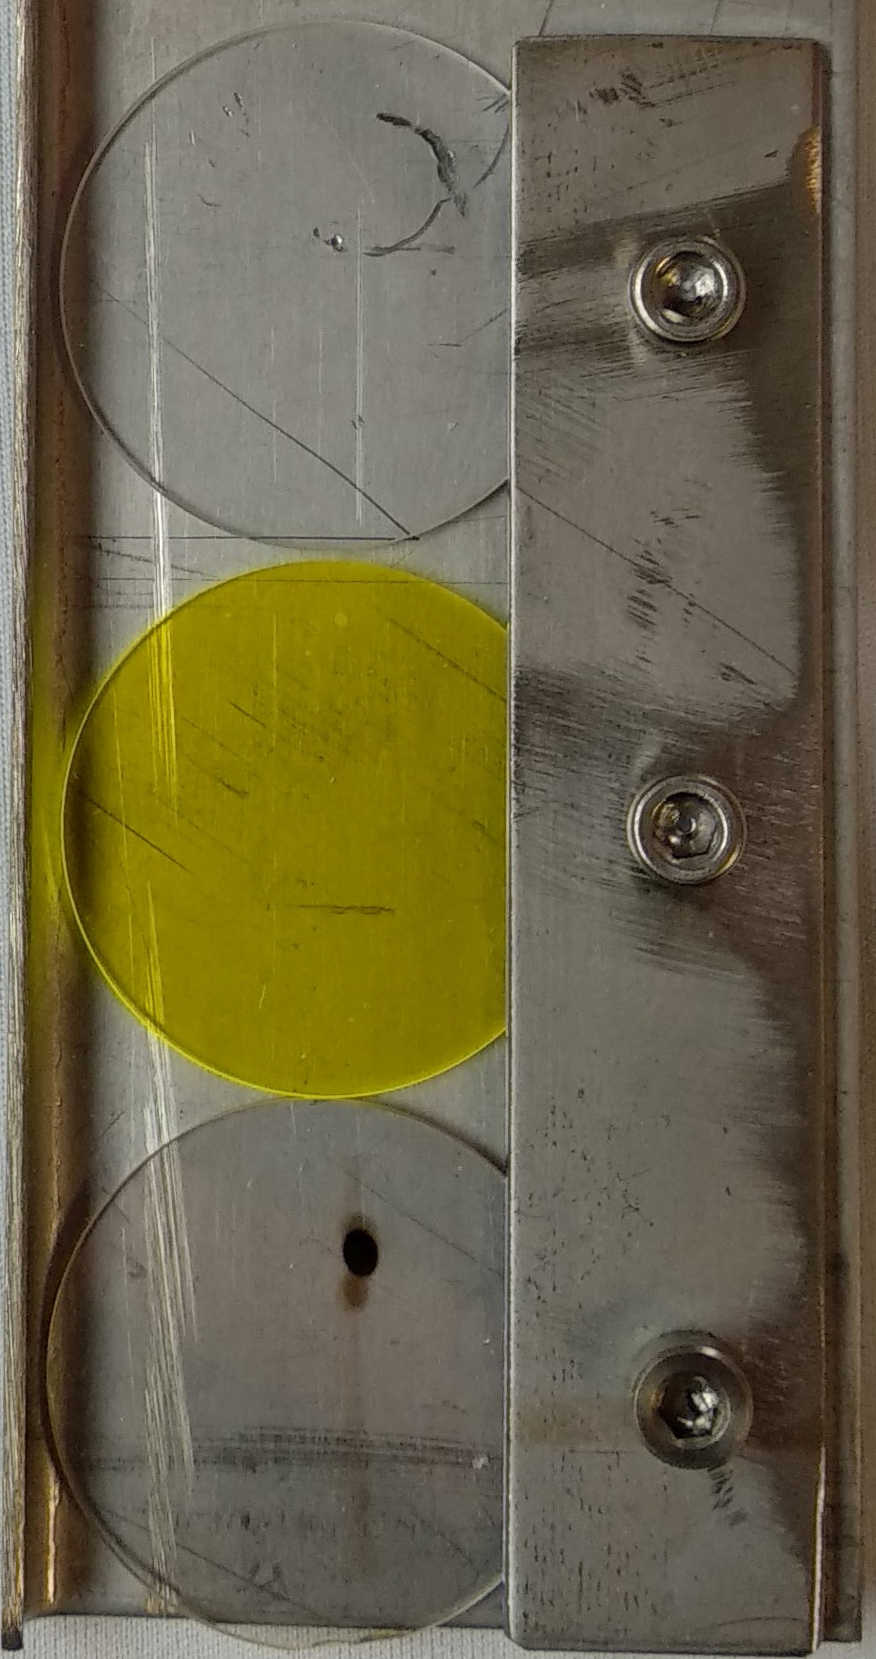
\includegraphics[width=0.3\textwidth]{04_IPHI_Test/figures/fig000_ecran.jpg}
  \caption[Picture of scintillator screen]{Picture of scintillator screen: Prelude420 (top), YAG:Ce (middle) and BGO (bottom).}
	\label{chap4:ecran}
\end{wrapfigure}


  \section{IPHI and test campaigns [C]}
  We had the opportunity to test our prototypes at IPHI accelerator twice. In the following sections, the accelerator and two campaigns are briefly introduced. Some pictures of the installation are shown in Fig. \ref{chap4:IPHI_tb}.

  \subsection{IPHI accelerator [C]}
  IPHI is a high intensity linear proton accelerator located at CEA/Saclay.
  This project has started in the late 90's\cite{Beau2000} but protons were accelerated up to $3\,\mathrm{MeV}$ MeV in April 2016\cite{Gobin2016}.

  Proton plasma is created by an electron cyclotron resonance source (ECR), and transported toward a radio frequency quadruple (RFQ) by a low energy beam transport line (LEBT).
  An iris ensures a fine tuning of the current, and two solenoids focus and filter the plasma before the injection in the RFQ.
  Then, the protons are accelerated up to $3\,\mathrm{MeV}$ and bunched with a frequency of $352\,\mathrm{MHz}$.
  A medium energy beam transport line (MEBT), downstream from the RFQ, contains focusing elements, steerers, dipole magnet and beam diagnostics.
  The dipole magnet can distribute the protons over two beam lines.

  \begin{figure}[!ht]
  \begin{center}
    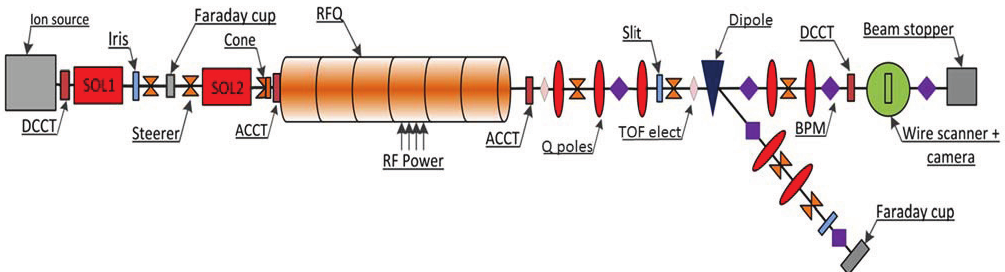
\includegraphics[width=\textwidth]{04_IPHI_Test/figures/fig000_IPHI_view.png}
  \end{center}
  \caption[Schematic view of IPHI accelerator]{Schematic view of the IPHI accelerator. The layout is almost up to date except that the slits have been removed. Our test bench was installed just after the last BPM on the deviated line.
    There is no other beam profiler measurement on this line.}
  \label{chap4:IPHI_view}
\end{figure}


  The main line has a dedicated beam stop of $300\,\mathrm{kW}$, allowing the commissioning of the accelerator at high intensity and duty cycle.
  The secondary line is more modular but restricted to beam at lower intensity and duty cycle (few hundred Watt).
  This line is open for external user experiments.
  We were, with the nBLM team, one of the first experiments on the deviated line\cite{Senee:IPAC2018-TUPAF016}.

  Fig. \ref{chap4:IPHI_view} shows a schematic view of the IPHI accelerator, and Table \ref{chap4:IPHI_carac} sums up the main differences between IPHI and ESS.
  \begin{table}[!h]
  \centering
  \caption[Comparison between IPHI and ESS accelerators]{Comparison between IPHI and ESS accelerators.}
  \label{chap4:IPHI_carac}
  \begin{tabular}{lll}
    \toprule
                         & IPHI accelerator                                  & ESS accelerator                \\
    \midrule
    Energy               & $3\,\mathrm{MeV}$                                 & $2\,\mathrm{GeV}$              \\ \hline
    Max current          & $100\,\mathrm{mA}$                                & $62.5\,\mathrm{mA}$            \\ \hline
    Max pulse duration   & up to DC                                          & $2.86\,\mathrm{ms}$            \\ \hline
    Max pulse repetition & -                                                 & $14\,\mathrm{Hz}$              \\ \hline
    Vacuum range         & $5\cdot10^{-7}$ to $1\cdot10^{-8}\,\mathrm{mbar}$ & $1\cdot10^{-9}\,\mathrm{mbar}$ \\
    \bottomrule
  \end{tabular}
\end{table}

  \subsection{Overview of the two test campaigns [C]}
  % TODO: Reformuler
  In this section, we also want to introduce the story behind our two test campaigns, and give an overview of issues we faced.
  The prototypes were not ready for the beginning of the first campaign.
  Hence, they were debugged on site, and we encountered many technical problems (sparks, readout sync).
  We finally got our first profile after some fixes on our prototypes, and by reducing the maximum operating voltage.
  However, our prototypes were not able to measure the beam profile each day, and we observed strange artifacts on our profile.
  We solved this problem by asking a fine tuning of the beam parameters by a beam physicist.
  We became even more confident with our detectors when BPM systems were switched on, see next section.

  \begin{figure}[!ht]
	\begin{subfigure}{0.5\textwidth}
		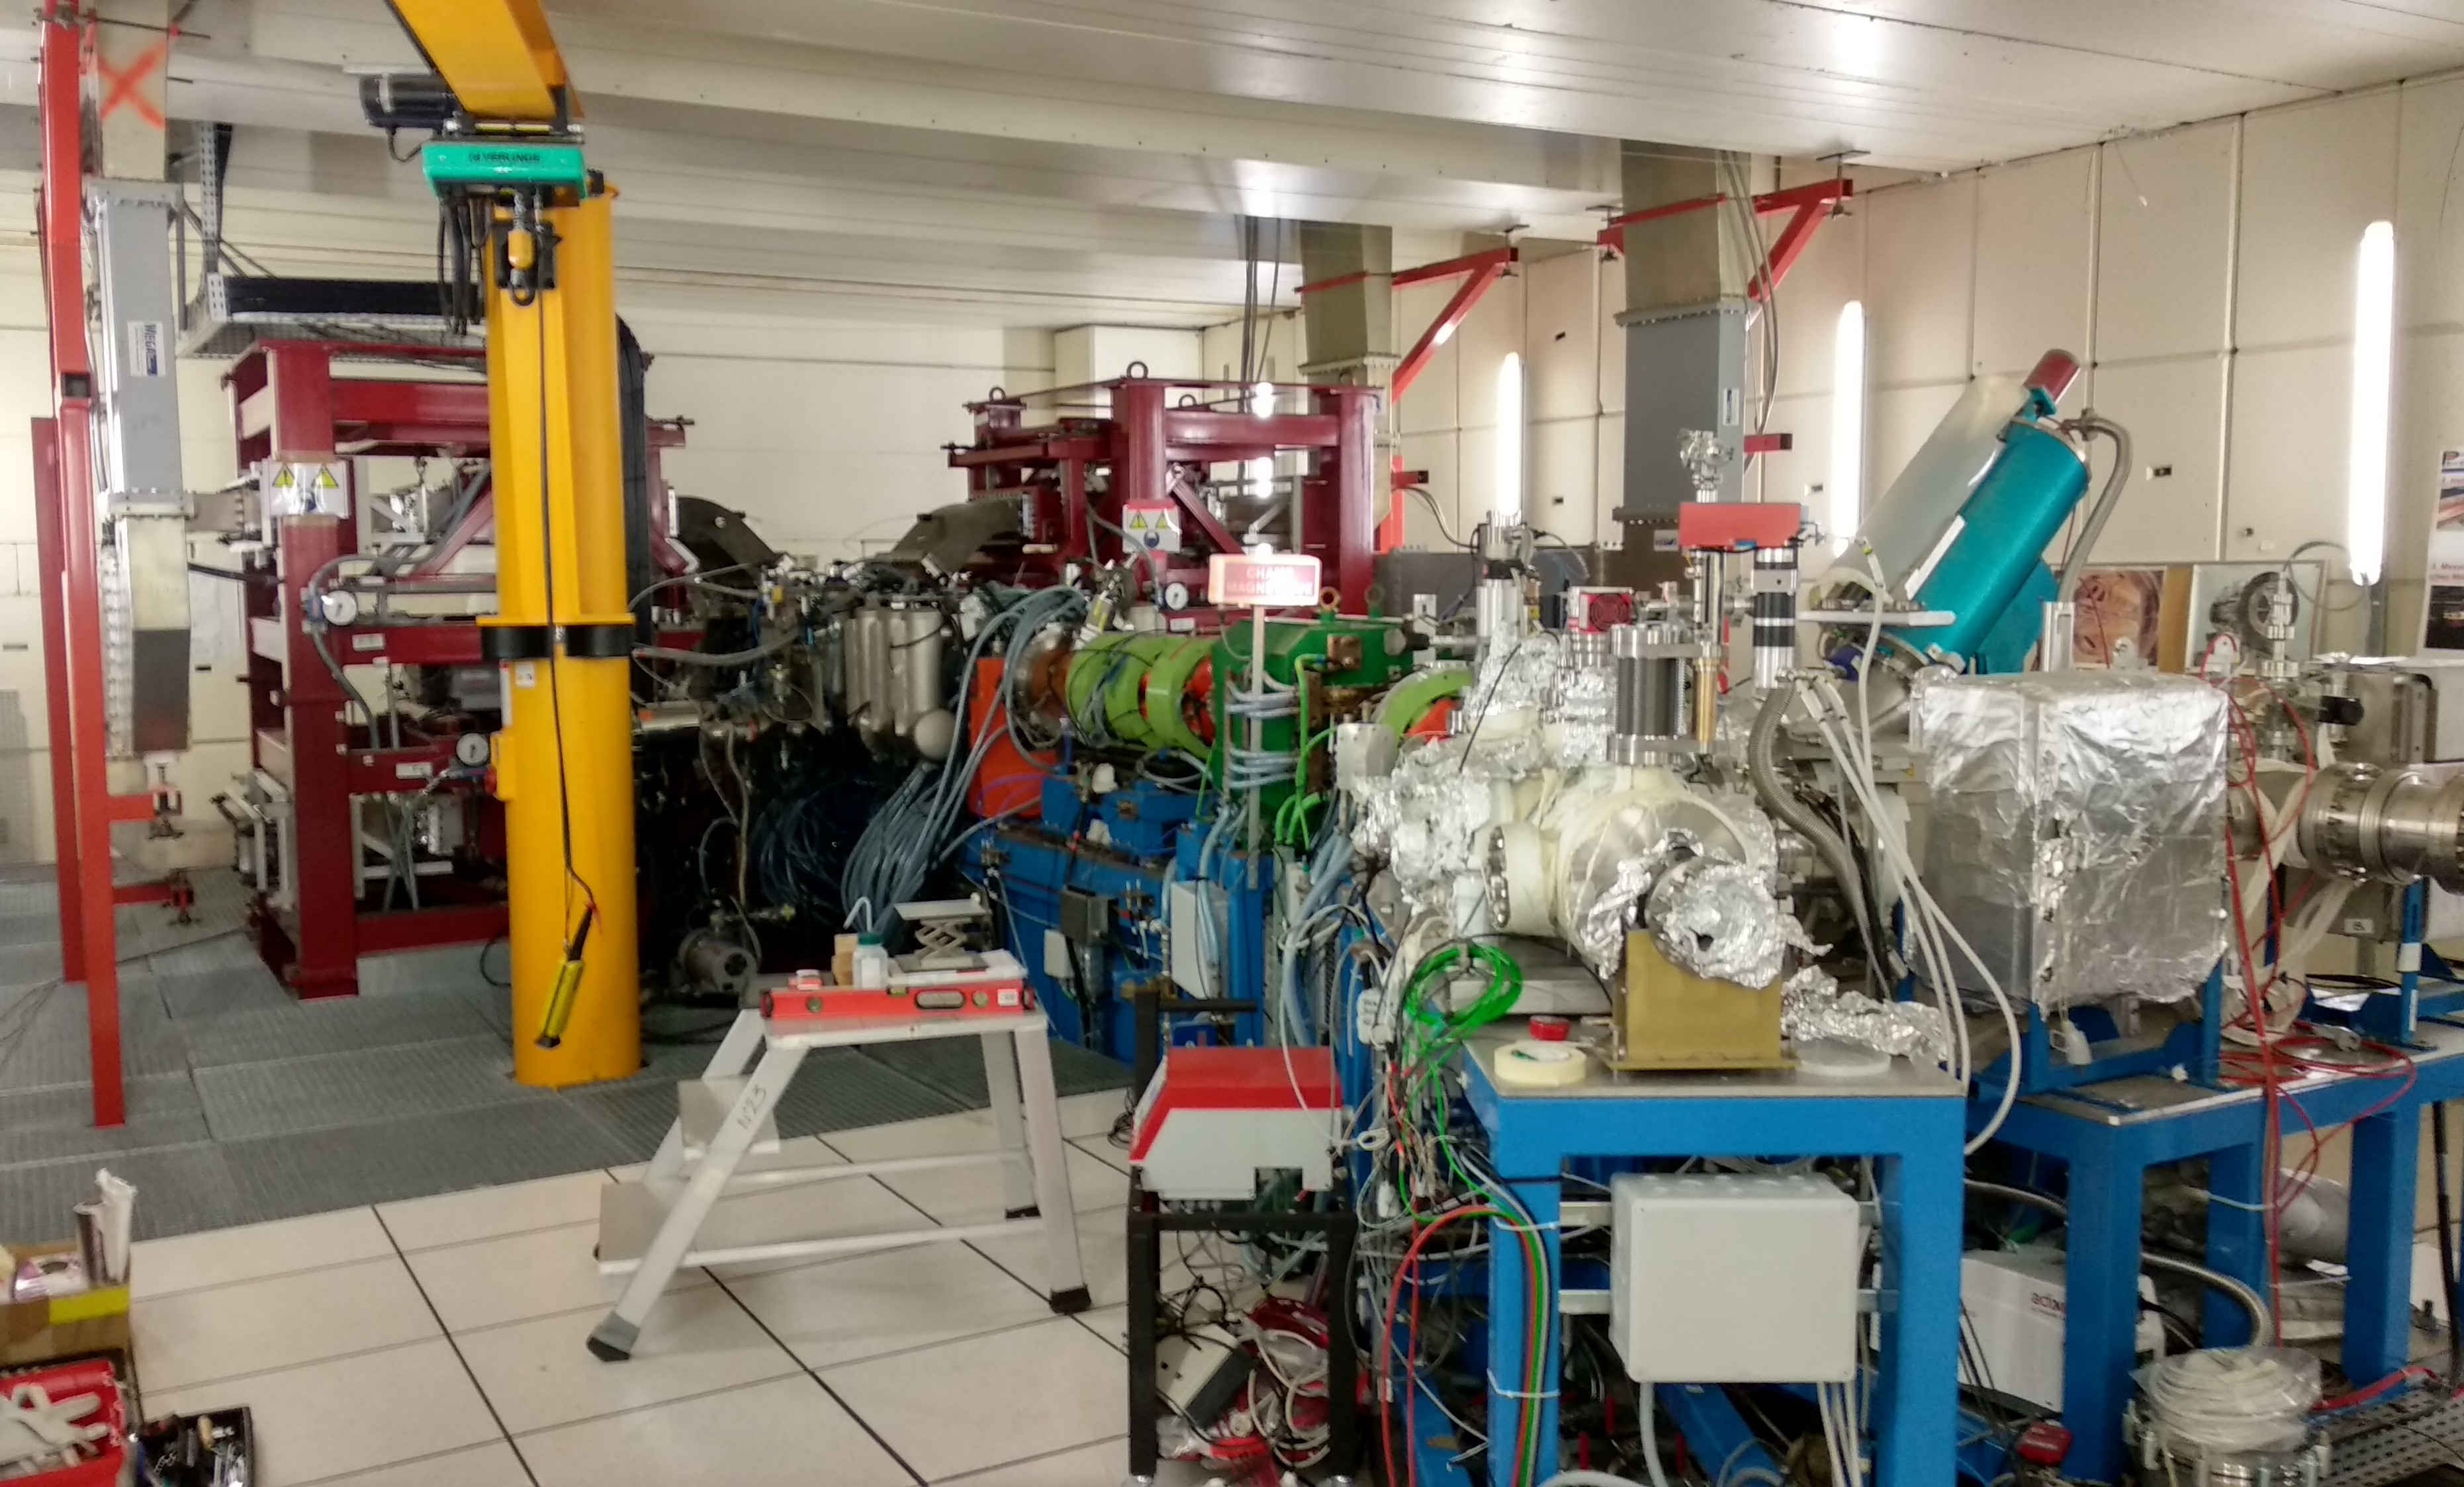
\includegraphics[width=\textwidth]{04_IPHI_Test/figures/fig000_IPHI_tb1.jpg}
		\caption{The casemate of IPHI. The test bench is visible in foreground}
		\label{}
	\end{subfigure}
	~
	\begin{subfigure}{0.5\textwidth}
		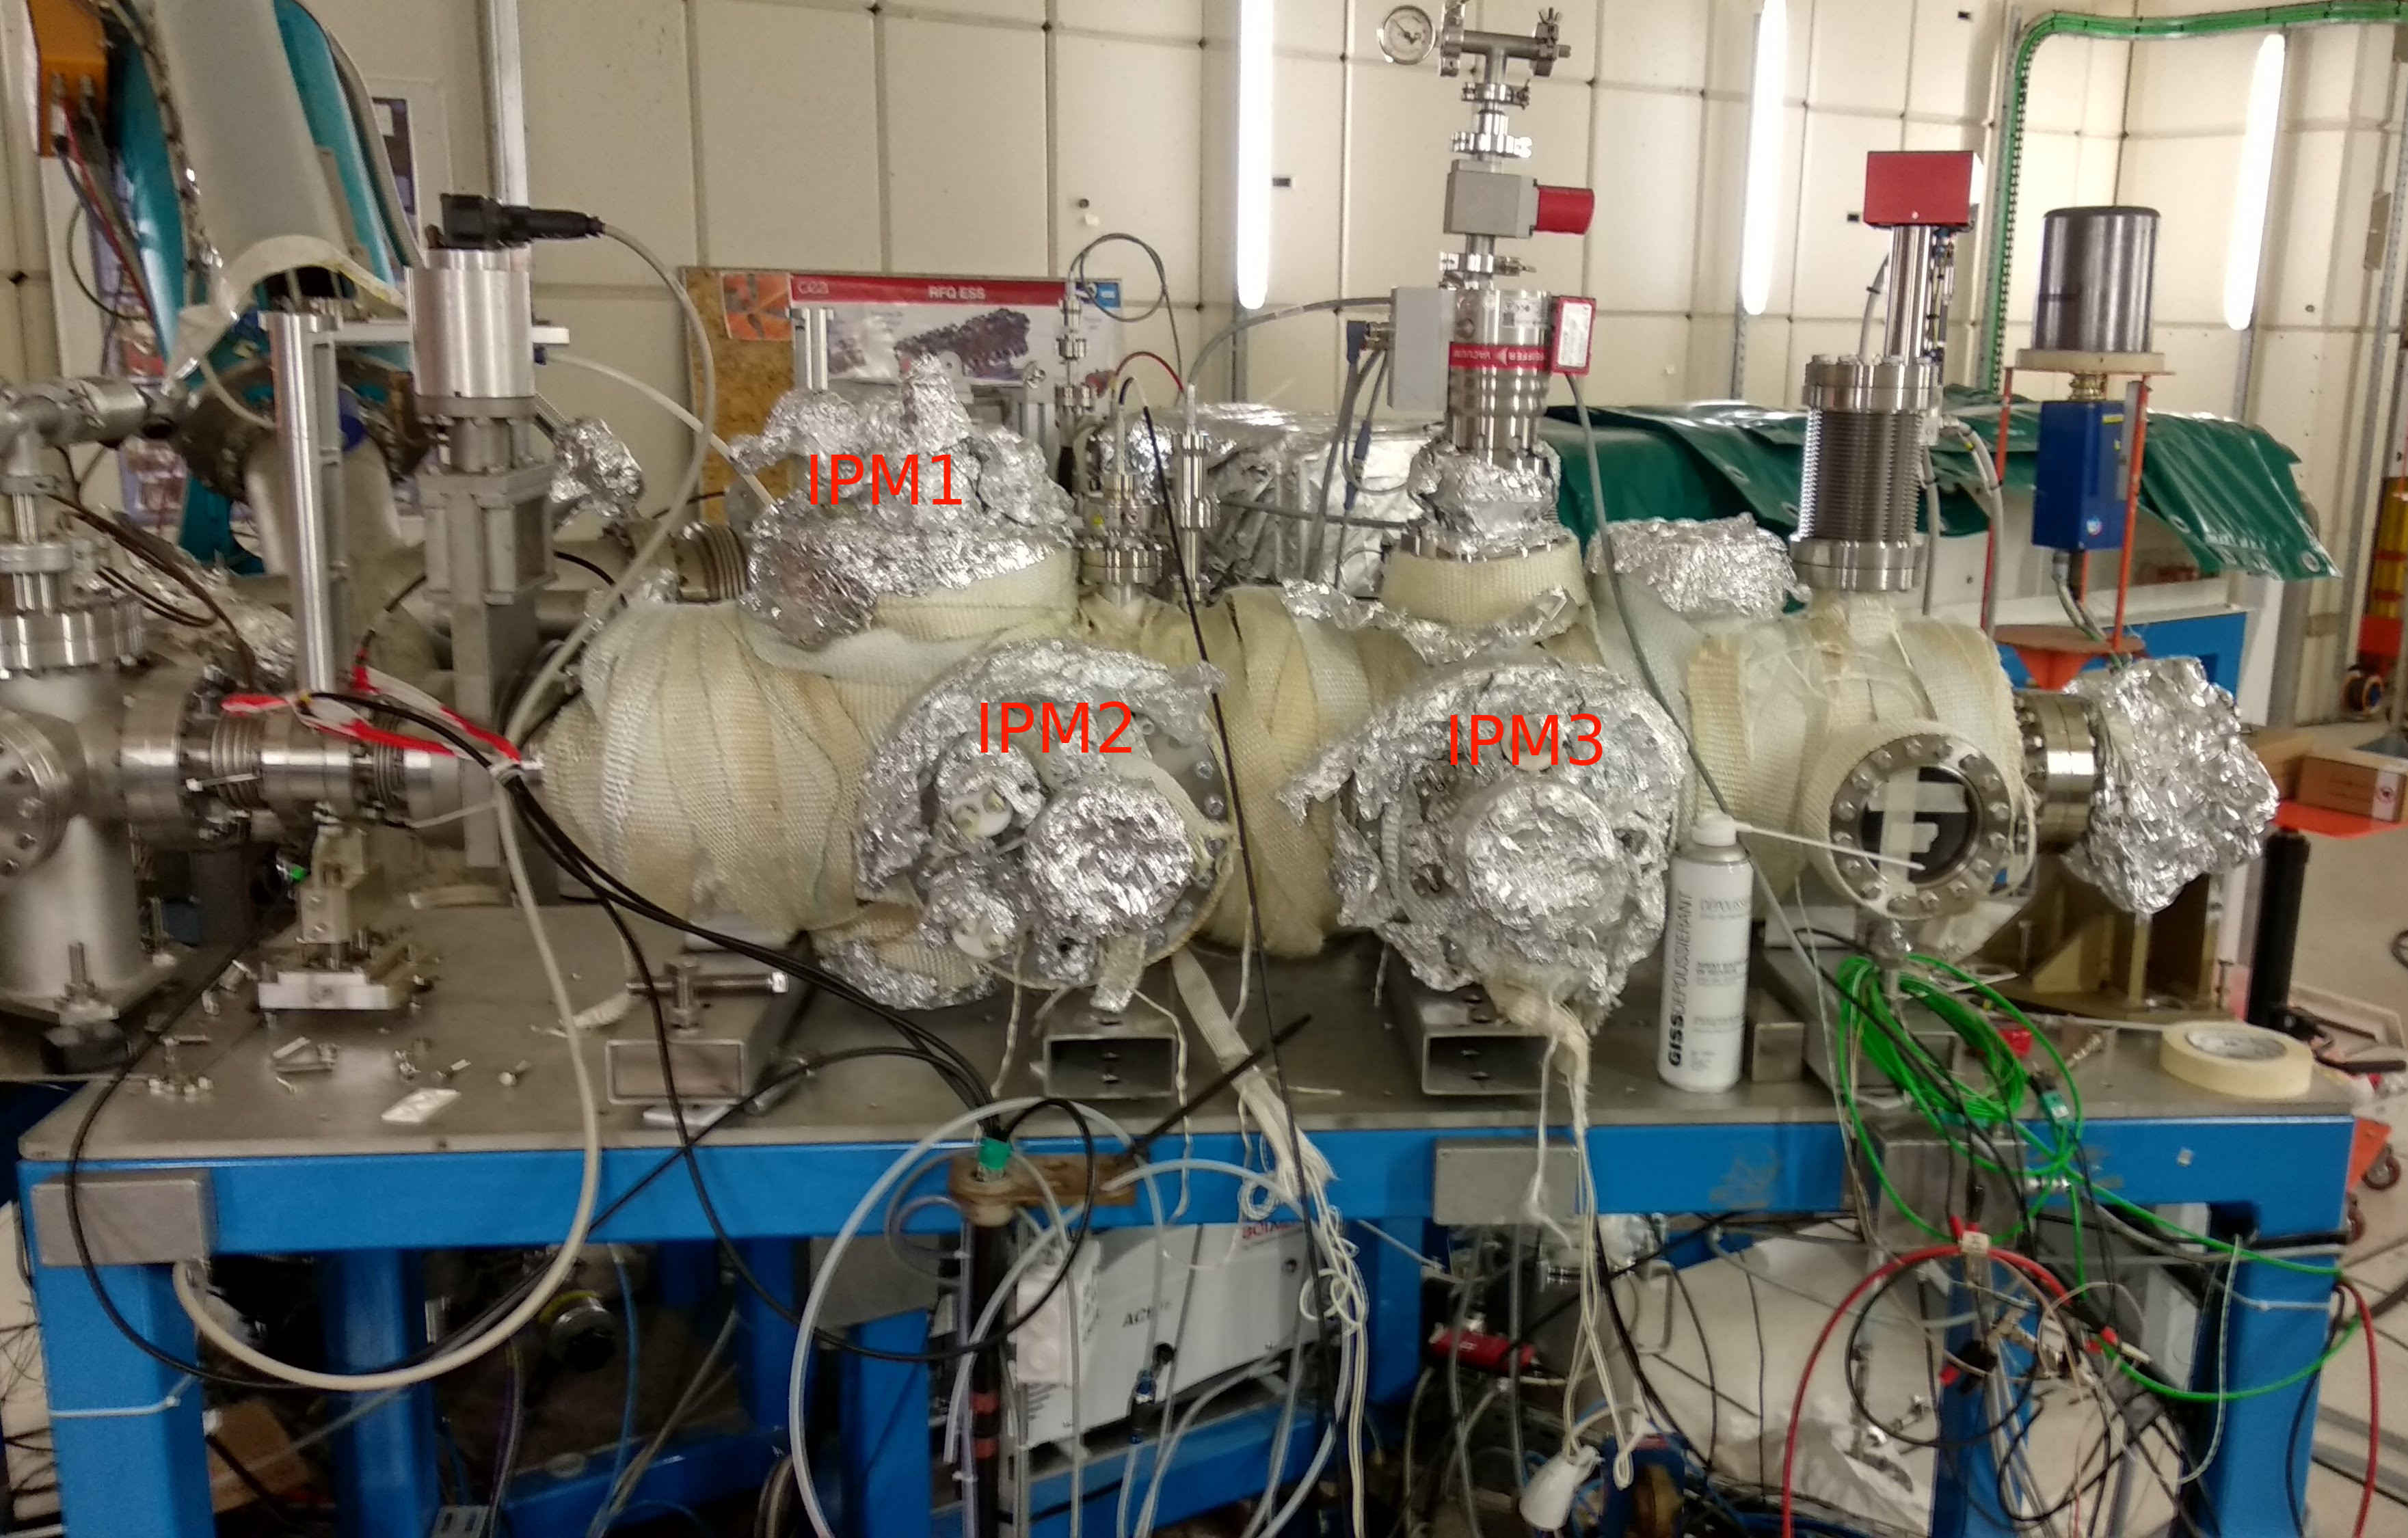
\includegraphics[width=\textwidth]{04_IPHI_Test/figures/fig000_IPHI_tb2.jpg}
		\caption{The test bench fully equipped.}
		\label{}
	\end{subfigure}
	\caption[The test bench installed at IPHI accelerator]{Th test bench installed at IPHI accelerator.}
	\label{chap4:IPHI_tb}
\end{figure}


  Just after the first campaign the detectors has been improved by minor changes on the HV connection design. Therefore, The decision has been made to perform a second test campaign at IPHI.
  The second campaign confirmed and improved our first results.
  The beam time was shared between four experiments, with each different requirements on the beam parameters.
  Unfortunately, the schedule was not respected due to technical problems and other external reasons, so
  we had to manage our tests daily and get along with the other experiments.
  On the other hand, we didn't manage to perform all advanced tests we planed to do.
  The Table \ref{chap4:IPHI_campaign} summarizes our two beam test campaigns

  \begin{table}[!h]
  \centering
  \begin{tabular}{ccc}
    \toprule
                  & First campaign      & Second campaign     \\
    \midrule
    Starting date & 19/02/2018          & 14/09/2018          \\
    First profile & 01/03/2018          & 14/09/2018          \\
    Ending date   & 13/04/2018          & 26/10/2018          \\
    IPM 1         & Linear strips (Y)   & Gaussian strips (X) \\
    IPM 2         & Hamamatsu MCP (Y)   & Photonis MCP (Y)    \\
    IPM 3         & Gaussian strips (Y) & Linear strips (Y)   \\
    \bottomrule
  \end{tabular}
  \caption[Summary of the two campaigns]{Summary of the two campaigns.}
  \label{chap4:IPHI_campaign}
\end{table}


  \section{Processing data [C]}
  In the following sections the data processing is briefly explained. Each method has its own characteristics so the data processing is a different depending on the IPM. The term beam size refers to the $\sigma_{beam}$ of the beam. The error bars in the following plots are given for a confidence level of $95\,\mathrm{\%}$. This assumes that the variation follows a normal distribution.

  \subsection{Processing camera [C]}
  The optical IPM gives directly an image of the beam in longitudinal and transverse direction. Thanks to EPICS and AreaDetector all images and related acquisition information are packed together in an HDF5 file. The processing of data is done with different Python packages \cite{NumPy2011,SciPy2019,Hunter2007}. In a first step, dead pixels are removed: the standard deviation of the image is computed and each deviating pixel is smoothed by a convolution filter. The algorithm works well if two dead pixels are not one beside to the other. Then, the image is cropped to a region of interest i.e. the active surface of the MCP.  If necessary, the image is filtered in frequency domain via a Fast Fourier Transform (FFT) \cite{Burrus2012}. FFT filtering is very efficient method since the images have many recurring pattern that are even visible by an human eye. However, at ESS it may not be the most suitable filter since the pattern will be more spatially dependant since the image may be comprised of small discrete spots rather than a continuous image. Therefore, more advanced method like wavelets \cite{Burrus1997,bultheel2014} should be forseen. Note that beam images are quite parsimonious in the frequency domain. The profile is reconstructed by summing all pixels in the longitudinal direction.

  \begin{figure}[!ht]
	\begin{center}
		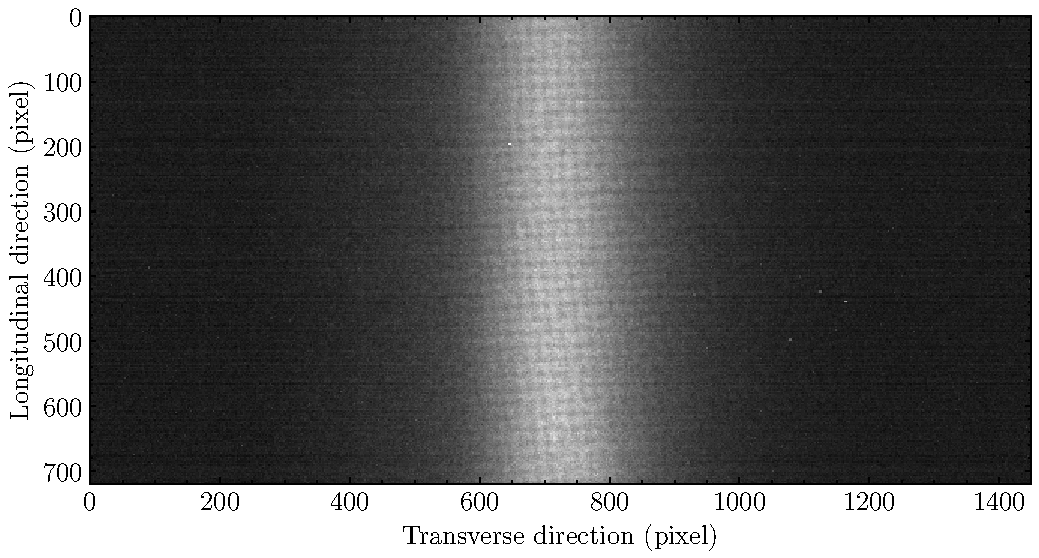
\includegraphics[width=\textwidth]{04_IPHI_Test/figures/fig000_image_beam}
	\end{center}
	\caption[An example of a beam image recorded by the camera]{An example of a beam image recorded by the camera. The image has just been cropped to a region of interest. The shadow of the grid is visible.}
	\label{chap4:image_beam}
\end{figure}


  \subsection{Processing strip [C]}
  The processing of data from strips is completely different and more complex. Indeed only a small part of the recorded signal is meaningful since the chips integrate continuously. The duration of the beam pulse was always short during the tests (from $50\,\mathrm{\mu s}$ to $1\,\mathrm{ms}$), therefore only a small amount of data is really useful.

  The data are processed as follows with ROOT\cite{Brun1997,Antcheva2009} routines. First, the pedestal of each strips is subtracted. If $N$ successive points are more than above a given threshold, then the pulse is considered as triggered. A pulse is detected when the previous condition is met on several strips at same time. Finally the successive $N$ integrations are summed giving the charge collected for one pulse. For Gaussian strips the charges are weighted according to the size of the strip.

  An example of a raw signal is given in the Fig. \ref{chap4:strips_signal}. On the left hand side, one can see the signal recorded during $45\,\mathrm{s}$. Each peak corresponds to the passage of the beam but does not correspond to the real signal. The signal for one pulse is visible on the right hand side.

  \begin{figure}[!ht]
  \begin{subfigure}{0.5\textwidth}
    \includesvg[width=\textwidth]{04_IPHI_Test/figures/fig000_strips_signal_a.svg}
    \caption{Full signal over a 45 sec.}
    \label{}
  \end{subfigure}
  ~
  \begin{subfigure}{0.5\textwidth}
    \includesvg[width=\textwidth]{04_IPHI_Test/figures/fig000_strips_signal_b.svg}
    \caption{Zoom on one pulse beam pulse.}
    \label{}
  \end{subfigure}
  \caption[Example of charge signal recorded on one strips]{Example of charge signal recorded on one strips.}
  \label{chap4:strips_signal}
\end{figure}



  \subsection{Processing scintillator screen and review on the reference measurements [C]}
  Scintillator screens can only operate at low duty cycles, typically some mA and few hundred us. Even under these conditions the beam destroyed two of the three screens. The signal is so strong that the camera in front of the screen is completely saturated, as well as the camera of the optical IPM one meter away. Measurements on the scintillator screens are only possible if a neutral filter is placed in front of the lens. The signal of screen completely overlaps the one of phosphorus screen and since we use monochromatic camera there is no way to recover beam profile from the optical IPM. For the strips IPM the working condition are already to low for a correct measurement. It is therefore not possible to compare the beam profile with the screens in real time.
  \begin{figure}[!ht]
	\begin{subfigure}[t]{0.3\textwidth}
		\includesvg[width=\textwidth]{04_IPHI_Test/figures/fig000_ScreenBeam_a}
		\caption{Image on screen}
		\label{}
	\end{subfigure}
	~
	\begin{subfigure}[t]{0.3\textwidth}
		\includesvg[width=\textwidth]{04_IPHI_Test/figures/fig000_ScreenBeam_b}
		\caption{Projection on $x$ axis}
		\label{}
  \end{subfigure}
  ~
  \begin{subfigure}[t]{0.3\textwidth}
		\includesvg[width=\textwidth]{04_IPHI_Test/figures/fig000_ScreenBeam_c}
		\caption{Projection on $y$ axis}
		\label{}
  \end{subfigure}
	\caption[Beam profile measurement with the $Y_{3}Al_{5}O_{12}(Ce)$ screen]{Beam profile measurement with the $Y_{3}Al_{5}O_{12}(Ce)$ screen.}
	\label{chap4:ScreenBeam}
\end{figure}

  Fig. \ref{chap4:ScreenBeam} shows an example of a profile measurement recorded on the $Y_{3}Al_{5}O_{12}(Ce)$ screen. The processing is almost the same as the optical IPM: hot pixels are corrected and the images are cropped. Then, a homography is performed to correct the orientation of the screens. The measurement of the beam size is quite complicated because the baseline of the profile is not straight, therefore the fits have a very poor quality. One can see that the profile is quite wide in the $x$-plane because of the dispersion due to the dipole. During the second campaign the dispersion was reduced by an small aperture located just after the dipole (?).

  The conditions are also not favourable for measurements with FPMs. The viewports are very close to the beam dump and when it stops the particles from the beam, stray light is emitted. The vacuum chamber (and the entire accelerator) allows light to propagate easily due to reflections on 304L steel. The vacuum is quite low so the expected signal is low. The beam power cannot be increased because it may create more stray light from beam dump. Our suspicions were confirmed when we added a sleeve with a black coating to shield the FPMs field view from the rest of the vessel. The parasitic light is shown in Fig. \ref{chap4:FPM}. It is clear that light enters through the openings. Many attempts to minimize these lights have been unsuccessful.

  \begin{figure}[!ht]
	\begin{center}
		\includesvg[width=0.5\textwidth]{04_IPHI_Test/figures/fig000_FPM}
	\end{center}
	\caption[Image recorded with the FPM system.]{Image recorded with the FPM system. The light coming from outside of the sleeve doesn't permit a correct measurement.}
	\label{chap4:FPM}
\end{figure}


  \section{Beam environnement characterization[En cours de rédaction]}
  First of all, it is necessary to present the experimental conditions under which our detectors have been characterized. One of the major problems encountered during these tests was the lack of information about the beam. The two types of diagnostics available at IPHI on the deviated line are current meters and BPMs whose calibration is uncertain. During the first weeks of the test campaign it was impossible for us to know if the strange things observed were due to the beam or the detectors themselves. The following measurements were made with our test bench.

  \subsection{Vacuum analysis [C]}
  \label{sec4:vacuum}
  During the tests, the vacuum parameters were recorded in real time \footnote{The vacuum gauge can provide a measurement at every pulse whereas a full RGA scan takes around two minutes}. However, neither the RGA nor the vacuum gauge has been calibrated. It is assumed that the RGA provides a qualitative information about the proportions of each species in the residual gas whereas the vacuum level is given more precisely by the vacuum gauge.

  There are two main types of RGA spectrum as shown in Fig. \ref{chap4:vacuum_rga}. The one, on right left side, are obtained when the chamber has not been baked or after an water contamination. As consequence the water peak dominated and the pressure is in the range of $10^{-7}\,\mathrm{mbar}$. After a few days of pumping or after drying, the RGA spectra tend towards the second case, on the right hand side. In this case the vacuum level is about $10^{-8}\,\mathrm{mbar}$ and the hydrogen is main specie. One can see some quite heavy elements on the two spectra, possibly oil residues. Indeed one of our turbo pumps was contaminated with oil from its old primary pump.

  \begin{figure}[!ht]
  \begin{subfigure}[t]{0.5\textwidth}
    \includesvg[width=\textwidth]{04_IPHI_Test/figures/fig000_vacuum_rga_a}
    \caption{An RGA spectrum dominated by water peaks.}
    \label{chap4:vacuum_rga_b}
  \end{subfigure}
  ~
  \begin{subfigure}[t]{0.5\textwidth}
    \includesvg[width=\textwidth]{04_IPHI_Test/figures/fig000_vacuum_rga_b}
    \caption{An RGA spectrum after few days of pumping or baking.}
    \label{chap4:vacuum_rga_a}
  \end{subfigure}
  \caption[Two types of RGA spectra recorded during the tests]{Two types of RGA spectra recorded during the tests.}
  \label{chap4:vacuum_rga}
\end{figure}


  When the beam is running, the pressure increases slightly as well as the amplitude of all the peaks in the RGA spectrum. We suppose that theses effects are mainly due to the heating of the beam dump. In the same way, the pressure increases when the resistance chains are fed, probably due to the Joule effect. On some RGA spectra, the hydrogen peak is subject to overshoots when the beam is running.

  \subsection{Beam position [C]}

  The first observation we made on the profile measurements was the significant variation of the beam position between two pulse. At first, we thought of an electrostatic discharge that could push the ionization byproducts during their drifts. However, this hypothesis was discarded when the BPM systems were restarted. For the first time, we were able to compare our measurement with another device. The Fig. \ref{chap4:BPMvsIPM} shows the position of the beam for about an hour recorded by IPM and BPM. The big sharp transitions are the consequences of moving the beam with electrostatic steerers. However, there are quite a few smaller variations between two steerer steps. A variation exceeding $2\mathrm{mm}$ ($5\mathrm{\%}$ of our readout size) can be observed from pulse to pulse. This is not a profile comparison but the same beam instabilities are visible on both devices.

  \begin{figure}[!ht]
	\begin{center}
		\includesvg[width=\textwidth]{04_IPHI_Test/figures/fig000_BPMvsIPM}
	\end{center}
  \caption[Beam position over the time measured with the BPM and the IPM]
  {Beam position over the time measured with the BPM and the IPM.
  A steerer has been used to move the beam (step transitions).
  However, small variations between two steerer steps were not expected. 
  Positions were directly extracted from IOCs without any processing.}
	\label{chap4:BPMvsIPM}
\end{figure}


  This is a major issue since MCPs have good space resolution but we were not allowed to fully benefit of this feature. All our measurement has been affected by those parasitic variations and therefore the level of confidence on the measurement is reduced. The histograms of beam size and position over 480 consecutive pulses are reported in Fig. \ref{}. One can see that both distribution are asymmetric and have similar shape. The linear regression between size and position has been calculated from several runs and shows an non-zero slope. On the other hand the correlation factor between size and position is not so high usually and vary between 0.5 and 0.8 from run to run.

  \begin{figure}[!ht]
  \begin{subfigure}[t]{0.5\textwidth}
    \includesvg[width=\textwidth]{04_IPHI_Test/figures/fig000_hist_variation_a.svg}
    \caption{Histogram of positions.}
    \label{}
  \end{subfigure}
  ~
  \begin{subfigure}[t]{0.5\textwidth}
    \includesvg[width=\textwidth]{04_IPHI_Test/figures/fig000_hist_variation_b.svg}
    \caption{Histogram of sizes.}
    \label{}
  \end{subfigure}
  \caption[Histograms of the beam positions and sizes for 480 consecutive pulses]{Histograms of the beam position and size for 480 consecutive pulses.}
  \label{chap4:hist_variation}
\end{figure}


  The main explanation given by IPHI experts about theses variation is that the beam may be more unstable when the pulse beam is short. However, we did not have time to confirm this hypothesis.

  \subsection{Beam current [C]}
  At IPHI the current is finely adjustable thanks to the iris but  IPHI has been designed to work at high current (above $50\mathrm{mA}$). On the other hand, to be in conditions close to those of ESS the current and duration of the pulse must be lowered. Varying the beam current is very important because it allows to check many properties of the detector. However, the shape of the IPHI beam changes greatly with current. This phenomenon is illustrated in Fig. \ref{chap4:ex_beam_profile_a} and \ref{chap4:ex_beam_profile_b}. When the currents are high, the beam looks like Gaussian with one of its shoulders more spread out. At medium and low current the size of the beam decreases as well as its amplitude. However, a kind of halo appears and this becomes more and more important as the current decreases. At very low current the beam core disappears completely and only the halo remains.

  \begin{figure}[!ht]
  \begin{subfigure}[t]{0.5\textwidth}
    \includesvg[width=\textwidth]{04_IPHI_Test/figures/fig000_ex_beam_profile_a.svg}
    \caption{At high current the beam looks almost Gaussian.}
    \label{chap4:ex_beam_profile_a}
  \end{subfigure}
  ~
  \begin{subfigure}[t]{0.5\textwidth}
    \includesvg[width=\textwidth]{04_IPHI_Test/figures/fig000_ex_beam_profile_b.svg}
    \caption{At low beam current, the beam shows a narrow peak on the top of a large halo.}
    \label{chap4:ex_beam_profile_b}
  \end{subfigure}
  \caption[Influence of the beam current on the beam shape.]{Influence of the beam current on the beam shape.}
  \label{chap4:ex_beam_profile}
\end{figure}


  This causes a problem because the beam shape is different depending on its intensity. The question is how to quantify the size of the beam. Several methods has been considered. One can simply calculate the mean value and standard deviation of the profile distribution but the results are strongly biased by the beam position and the asymmetric shape of the profile. A more advanced method consists in performing a curve-fitting of the profile with a Gaussian function for recovering the estimated sigma. The method works quite well at high currents but at low currents the halo prevents the beam from splitting correctly. To overcomes this issue, a second Gaussian function can be added to the fitting routine. The double fit succeeds in correctly modeling the two components. However, double fits may modelize almost any beam shape and the fitting results are difficult to verify automatically. The method becomes very unstable for high currents. This is why it must be limited to the low current. The last alternative is to use the full width at half magnitude (FWHM). Assuming that the beam is more or less Gaussian, the sigma can be calculated as follow $\sigma = \frac{FWHM}{\sqrt{2ln(2)}}$. It is easy to implement and very fast compared to fits.

  \begin{figure}[!ht]
  \begin{subfigure}[t]{0.5\textwidth}
    \includesvg[width=\textwidth]{04_IPHI_Test/figures/fig000_current_sweep_a}
    \caption{Integrated signal versus beam current. The blue curve represents the sum of the two components.}
    \label{}
  \end{subfigure}
  ~
  \begin{subfigure}[t]{0.5\textwidth}
    \includesvg[width=\textwidth]{04_IPHI_Test/figures/fig000_current_sweep_b}
    \caption{Sizes of the beam and halo versus beam current.}
    \label{}
  \end{subfigure}
  \caption[Influence of the beam current on the profile measurement.]{Influence of the beam current on the profile measurement.}
  \label{chap4:current_sweep}
\end{figure}


  Here the double fitting routine was used to monitor the evolution of the two components of the beam. First, the phenomenon described above is clearly visible. At high current the signal tends towards a Gaussian shape, whereas at low current the double Gaussian model seems more realistic. Secondly, the amplitude of the signal is linear with the beam current. At high currents the input signal on the MCP is several orders of magnitude above the expected signal at ESS. This means that there will be no saturation at ESS with a single-stage MCP.

  \subsection{Beam tuning [C]}
  The beam tuning is also important to insure a correct measurement of the profile. IPHI line contains many beam optic elements to control the beam transport. An incorrect adjustment of the beam has significant consequences on the quality of our measurements. Indeed, during the first weeks of testing we could not have stable and reproducible measurements. Some days the profiles were quite clean while the next days profiles showed strange artifacts. An example is given in Fig. \ref{chap4:beam_tuning_a}. One can see that the profile is visible in the image two but with two spots on each side. We have no explanation about the origin or nature of these spots. They disappear completely when the beam is properly adjusted.
  
  The optimal parameters were found thank to a beam physicist and the TraceWin software software. In practice, the beam has been adjusted to have the lowest possible convergence at along test bench. The beam size has been tuned  in similar (few mm) with the different quadrupoles (Fig. \ref{chap4:beam_tuning_b}). Once the beam was adjusted, all the parameters were frozen. This allowed us to measure the profile correctly.

  \begin{figure}[!ht]
  \begin{subfigure}[t]{0.5\textwidth}
    \includesvg[width=\textwidth]{04_IPHI_Test/figures/fig000_beam_tuning_a}
    \caption{A poorly beam tune leads to strange signal on the top of the image.}
    \label{chap4:beam_tuning_a}
  \end{subfigure}
  ~
  \begin{subfigure}[t]{0.5\textwidth}
    \includesvg[width=\textwidth]{04_IPHI_Test/figures/fig000_beam_tuning_b}
    \caption{The beam size can be set at different size thank to quadrupoles.}
    \label{chap4:beam_tuning_b}
  \end{subfigure}
  \caption[The beam must be finely tune in order to perform correct measurements]{The beam must be finely tune in order to perform correct measurements.}
  \label{chap4:beam_tuning}
\end{figure}


  %\input{04_IPHI_Test/figures/fig000_position_sweep}

  \section{IPM characterization [C]}
  In the next sections the most common aspects of IPMs are presented. The goal is to collect as much information as possible about the detectors and their limitations to prepare the final design. Most of the data presented below come from optical IPMs. Unfortunately, many of the acquisitions done with the strips were polluted by noise and strange behaviour with the electronics.

  \subsection{High voltage and Space Charge verification [En cours de rédaction]}
  [Mettre une image SC ?]

  \begin{figure}[!ht]
	\begin{center}
		\includesvg[width=\textwidth]{04_IPHI_Test/figures/fig000_HT_size}
	\end{center}
	\caption[]{}
	\label{chap4:}
\end{figure}


  \subsection{Cross interaction [En cours de rédaction]}

  In the previous chapter we showed that the profile measurement can be greatly affected by the cross interaction between two close IPMs. The easiest solution to implement is to put disks connected to ground between each IPM, so each IPM is completely isolated from the other. The first part of the test chamber was built almost identical to the ESS LWU vessel. It is therefore possible to verify that the influence of one IPM on the other in almost ESS conditions. To check this, one IPM is switched on while the other is measuring the position and size of the beam. However, the measurement is not so simple for the second IPM. Indeed, at IPHI the protons of 3 MeV can be deflected by the extraction field of the IPMs. Therefore, we may measure the deviation of the pulse instead of the cross interaction. Fig. \ref{} shows the variations of beam position (right) and size (left) measured by IPM2 for different values of extraction field in the IPM1. The red curve exposes the theoretical deviation calculated from the voltage applied to the IPM1. The variation in beam size seems negligible, about $75,\mathrm{\mu m}$. On the other hand, the variation for the position is quite important, but the observed values are very close to the theoretical curve.
  [A voir si on a les courbes pour confirmer]

  \begin{figure}[!ht]
  \begin{subfigure}[t]{0.5\textwidth}
    \includesvg[width=\textwidth]{04_IPHI_Test/figures/fig000_cross_position}
    \caption{Variation of the beam position.}
    \label{chap4:cross_position}
  \end{subfigure}
  ~
  \begin{subfigure}[t]{0.5\textwidth}
    \includesvg[width=\textwidth]{04_IPHI_Test/figures/fig000_cross_size}
    \caption{Variation of the beam size.}
    \label{chap4:cross_size}
  \end{subfigure}
  \caption[Cross interaction between two IPMs.]{Cross interaction between two IPMs.}
  \label{chap4:cross}
\end{figure}


  \subsection{Comparison size [En cours de rédaction]}
  The IPHI beam may be deflected by the extraction fields of the different IPMs, in consequence most of the studies has been performed on an IPM one at a time. However some measurements requires to use both IPMs at the same time. For instance comparisons between the profiles measured by the two different IPM types. This is the only way to check the correctness of the measurement since there were no reference method working correctly during the tests.
  The superposition of the profile measured with the strips IPM and optical IPM one is shown in Fig. \ref{}. The strips IPM directly measure a number of charges whereas the camera gives a digital pixel value. The conversion factors of each element in the optical IPM have not been quantified, therefore the signal amplitude from camera data is only scaled, but the x-axis remains unchanged.

  [Mettre image comparison avec les strips]
  \begin{figure}[!ht]
	\begin{center}
		\includesvg[width=\textwidth]{04_IPHI_Test/figures/fig000_MCP_strips}
	\end{center}
	\caption[Superposition of the same beam profile measured with strips IPM and optical IPM]{Superposition of the same beam profile measured with strips IPM and optical IPM. The beam size measurements are in good agreament. The beam position can not be compared due to the beam angle induced by the steerers.}
	\label{chap4:MCP_strip}
\end{figure}


  \subsection{COMSOL simulation [C]}
  Simulations have been performed with COMSOL to cover both cases of asymmetric and symmetric configurations. The simulations expose a good uniformity with a  better result for symmetric configuration. However, it may be difficult to since the beam cannot be moved in a non uniform areas of the detector.

  A possible workaround consists in intentionally reduce the uniformity of the extraction, and the beam size and position will be more affected by non-uniformities. The optical IPM has been used in asymmetric configuration with a resistor chain designed for symmetric usage. Since resistor chains are different between asymmetric and symmetric configurations the extraction field will be also different. The electric field in this peculiar configuration can be simulated with COMSOL as shown previously.

  The three main effects have been observed from the simulations. Firstly, the beam image is smaller than the real beam size. This focusing effect is constant over the overall plane detection. Secondly, the extraction field tends to pull the beam image in the center of the detector. This effect is linear and null at the IPM center. Thus, the measured displacement is less important on the readout than the reality. Lastly, the beam image intensity is smaller in asymmetric because some particles are lost in the longitudinal direction. However, this effect can not be measured because the gain of MCP is not perfectly know on symmetric configuration and cannot be recovered correctly.

  We measured the beam size and displacement for several steerer values in the symmetric and asymmetric configurations.
  The extraction fields were set to a same value for both configurations and all other parameters were frozen. If we suppose that the symmetric mode gives the real beam position and size, hence it is possible to quantify the difference between the simulated and experimental values.

  % TODO: Commenter résultats
  For several value of extraction fields in both asymmetric and symmetric mode, the mean value of the slope of the beam displacement has been computed and compared with the results from simulations, see Fig. \ref{chap4:COMSOL_check_a}. In a same way the average ratio between beam size in symmetric and asymmetric configuration has been measured for several position and the comparisons with simulations is shown in Fig. \ref{chap4:COMSOL_check_b}.

  \begin{figure}[!ht]
  \begin{subfigure}{0.5\textwidth}
    \includesvg[width=\textwidth]{04_IPHI_Test/figures/fig000_COMSOL_check_a}
    \caption{}
    \label{}
  \end{subfigure}
  ~
  \begin{subfigure}{0.5\textwidth}
    \includesvg[width=\textwidth]{04_IPHI_Test/figures/fig000_COMSOL_check_b}
    \caption{}
    \label{}
  \end{subfigure}
  \caption[]{ }
  \label{chap4:COMSOL_check}
\end{figure}


  Note that the steerer was not able to cover the full range in position, but we preferred not using the dipole magnet to continue the scanning since it may affect the beam size.

  The method is clearly not perfect but it allows to reduce the IPHI uncertainty since it can be done without stopping down the accelerator.

  \subsection{Grid [C]}

  Due to the variations at IPHI it is difficult to determine the resolution on size and position obtained with the optical IPM. It depends greatly on the run considered and in the best case\footnote{For 480 consecutives pulses.} the confidence interval at $95\,\mathrm{\%}$ is about $\pm 5\,\mathrm{\mu m}$ on the beam size and  $\pm 30\,\mathrm{\mu m}$. There is also no reference measurement to compare results.

  However, we can try to quantify the spatial resolution of the MCP system and the camera.
  To measure this resolution, the grid can be used. By increasing the transmission as described in the section \ref{chap3:sec:grid} it is possible to significantly increase the contrast of the grid shadow as shown in Fig. \ref{chap4:grid_res_a}. Then, the Fourier transform is used to identify the harmonics due to the grid. The resulting Fourier image is visible in Fig. \ref{chap4:grid_res_b}. The beam signal is located in the center of the image in an small area ($20$ by $20$ pixels). The other spots that are repeated vertically and horizontally are due to the grid. The peaks closest to the center of the image are the lowest harmonics and it is possible to discriminate between them if their spacing exceeds 5 pixels or about $58.6\,\mathrm{\mu m}$. With this kind of spatial resolution and assuming that the beam that the beam does not vary as at IPHI, it is quite possible to achieve the resolution requested by ESS on the pulse position about $50\,\mathrm{\mu m}$. However, this result would probably be different with a two-stage MCP that tends to do more diffuse tasks on the phosphorescent screen.

  \begin{figure}[!ht]
  \begin{subfigure}{0.5\textwidth}
    \includesvg[width=\textwidth]{04_IPHI_Test/figures/fig000_grid_res_a}
    \caption{}
    \label{}
  \end{subfigure}
  ~
  \begin{subfigure}{0.5\textwidth}
    \includesvg[width=\textwidth]{04_IPHI_Test/figures/fig000_grid_res_b}
    \caption{}
    \label{}
  \end{subfigure}
  \caption[]{ }
  \label{chap4:}
\end{figure}


  \subsection{MCP [C]}
  The MCPs have been characterized directly with the IPHI beam, we did not have time to carry out studies before the beam tests. Therefore, we had no information about MCPs before their uses in real beam conditions.

  The main characteristic of a MCP is its gain. We cannot give the absolute gain of the MCP since the optical IPM were not calibrated. The signal on the camera was integrated for several MCP voltage from 600V to 1200V. The current of the beam was set to low value in order to not saturate the camera at high MCP gain. Fig.\ref{MCP_gain_a} exposes the relative gain of the MCP and a dynamic of 300 for the considered range. The total range of a MCP is between 600V and 1200V so we can expect an absolute dynamic range of 1000.

  The influence of the MCP gain on the beam size has been checked. However the beam current must at sufficient level in order to obtain an acceptable shape. On the other hand, the camera will  saturated more easily at high gain. Consequently, the range of the measurement is smaller than previously. This study is presented in Fig. \ref{MCP_gain_b}. The slope of the linear regression shows can be considered as null meaning that the gain doesn’t afflict the beam size. This tests has been done on both MCP

  \begin{figure}[!ht]
  \begin{subfigure}[t]{0.5\textwidth}
    \includesvg[width=\textwidth]{04_IPHI_Test/figures/fig000_MCP_gain_a.svg}
    \caption{Relative gain curve.}
    \label{MCP_gain_a}
  \end{subfigure}
  ~
  \begin{subfigure}[t]{0.5\textwidth}
    \includesvg[width=\textwidth]{04_IPHI_Test/figures/fig000_MCP_gain_b.svg}
    \caption{Influence of the MCP gain on beam size.}
    \label{MCP_gain_b}
  \end{subfigure}
  \caption[Characterization of the MCPs]{Characterization of the MCPs.}
  \label{chap4:MCP_gain}
\end{figure}


  \subsection{Phosphorus screens [C]}
  A phosphorus screen converts a charged particle into visible photons.
  The signal amplitude depends on the energy deposition of the particle in the phosphorus layer. In our case, the phosphorus screen is placed just after the MCP output.

  \subsubsection{Gain [C]}
  The signal is proportional to the accelerating voltage between the MCP output and the phosphorus screen. Two screens have been tested during the beam tests: the P43 and the P46. Each screen has its intrinsic characteristics like the yield, the emission wavelength and the decay time. Fig. \ref{fig:phos_integral} shows the linear response with the voltage for both the screens. According to Hamamatsu, the lifetime of a phosphorus screen is negligible with respect to the MCP lifetime.

  \begin{figure}[!ht]
	\begin{subfigure}[t]{0.5\textwidth}
		\includesvg[width=\textwidth]{04_IPHI_Test/figures/fig000_P43_size.svg}
		\caption{P43 screen.}
		\label{}
	\end{subfigure}
	~
	\begin{subfigure}[t]{0.5\textwidth}
		\includesvg[width=\textwidth]{04_IPHI_Test/figures/fig000_P46_size.svg}
		\caption{P46 screen.}
		\label{}
	\end{subfigure}
	\caption[Beam size versus phosphorus screen voltage.]{Beam size versus phosphorus screen voltage. No significant change of the beam size has been observed.}
	\label{chap4:P_size}
\end{figure}


  The important thing to check that there is no influence between the gain and the measured size and position. The beam size seems to be not affected by the screen gain for both screen, as depicted on Fig. \ref{fig:phos_pos}.

  \begin{figure}[!ht]
	\begin{subfigure}{0.5\textwidth}
		\includesvg[width=\textwidth]{04_IPHI_Test/figures/fig000_P43_gain.svg}
		\caption{}
		\label{}
	\end{subfigure}
	~
	\begin{subfigure}{0.5\textwidth}
		\includesvg[width=\textwidth]{04_IPHI_Test/figures/fig000_P46_gain.svg}
		\caption{}
		\label{}
	\end{subfigure}
	\caption[]{}
	\label{chap4:P_gain}
\end{figure}

  \subsubsection{Timing [C]}
  The measurement of decay time has been performed by moving the camera trigger at small exposure times. The measurement is a bit more difficult for the fast screen. Indeed, the exposure time is now comparable to the decay time, also the delay and the jitter on the exposure time may afflict the measurement.
  We measured for the PointGrey camera a delay of $25\,\mathrm{\mu s}$ and a jitter on the exposure time more than $50\,\mathrm{\mu s}$. The measurements for both screen is shown in \ref{chap4:P_timing}

  \begin{figure}[!ht]
	\begin{subfigure}{0.5\textwidth}
		\includesvg[width=\textwidth]{04_IPHI_Test/figures/fig000_P43_timing.svg}
		\caption{}
		\label{}
	\end{subfigure}
	~
	\begin{subfigure}{0.5\textwidth}
		\includesvg[width=\textwidth]{04_IPHI_Test/figures/fig000_P46_timing.svg}
		\caption{}
		\label{}
	\end{subfigure}
	\caption[]{}
	\label{chap4:P_timing}
\end{figure}

  As expected, the P43 is slow, thus if this screen is used for ESS then the total integration time on camera should be set to $10\,\mathrm{ms}$ and not strictly to $2.86\,\mathrm{ms}$. This is not the case with the P46 screen.

  \subsection{Detection limits with strips [En cours de rédaction]}

  \subsection{Extrapolation to ESS condition [C]}
  Unlike the strips IPM, it is almost impossible to quantify the number of ionization particles without a full calibration of the MCPs. Hence, the extrapolation to ESS conditions is only done from Bethe formula, with respect to the beam parameters and vacuum conditions measured at IPHI.
  However the MCP does not suffer of any bandwidth limitation as long as it is not saturated. The exposure time on camera has been set to $3\,\mathrm{ms}$ in order to get realistic electronic noise in the CMOS sensor.
  We supposed that the signal scales linearly with pressure. The beam current and the pulse duration were set to their lowest value possible at IPHI, respectively $0.7\,\mathrm{mA}$ and $50\, \mathrm{\mu s}$. The vacuum level was about $4 \cdot 10^{-8}\,\mathrm{mbar}$ and its composition was mainly water (conservative assumption), see section \ref{sec4:vacuum}. Table \ref{chap4:extrapolationMCP} sums up the factor of each parameter on the extrapolation.
  \begin{table}[ht]
  \centering
  \caption[Extrapolation to ESS conditions from a real case during the second campaign]
  {Extrapolation to ESS conditions from a real case during the second campaign.
    The IPHI current was below $0.7\,\mathrm{mA}$ with a pulse duration of $50\, \mathrm{\mu s}$. Pressure level was $4 \cdot 10^{-8}\,\mathrm{mbar}$ with mainly water vapors (conservative hypothesis).
    The scaling factor for each parameter is calculated from the nominal ESS beam conditions given in Table \ref{chap2:ess_charac}.}
  \label{chap4:extrapolationMCP}
  \begin{tabularx}{\linewidth}{XXXXXXX}
    \toprule    ESS energy (MeV) & Bethe Bloch & Pressure     & Gas composition & Intensity & Pulse length & Total         \\
    \midrule
    \(97.2\)                     & $\times 15.5$ & $\times 40 $ & $\times 2.2$    & $\div89$  & $\div57$     & $\times 0.27$ \\
    \(231.4\)                    & $\times 16.4$ & $\times 40$  & $\times 2.2$    & $\div89$  & $\div57$     & $\times 0.28$ \\
    \(278.9\)                    & $\times 29.9$ & $\times 40$  & $\times 2.2$    & $\div89$  & $\div57$     & $\times 0.52$ \\
    \(315.8\)                    & $\times 33.4$ & $\times 40$  & $\times 2.2$    & $\div89$  & $\div57$     & $\times 0.58$ \\
    \(628.3\)                    & $\times 35.8$ & $\times 40$  & $\times 2.2$    & $\div89$  & $\div57$     & $\times 0.62$ \\
    \bottomrule
  \end{tabularx}
\end{table}

  Fig. \ref{chap4:limits_IPHI} shows a example of a beam image and corresponding profile acquired in such conditions. As explained in the section, at really low current the beam is completely overlapped by the halo component. The signal on image looks more discrete with several spots. Indeed, at this current some channels are no more hit every pulse. Each sport may be related to a hit on a single channel.
  % TODO: Commenter l'image
  At first glance, it seems to be possible to measure single profile at nominal ESS conditions. However, this assumption is strongly dependent to the vacuum conditions. Neither the RGA nor the gauges were calibrated, so the uncertainty may be relevant.

  \begin{figure}[!ht]
  \centering  
  \begin{subfigure}[t]{1\textwidth}
    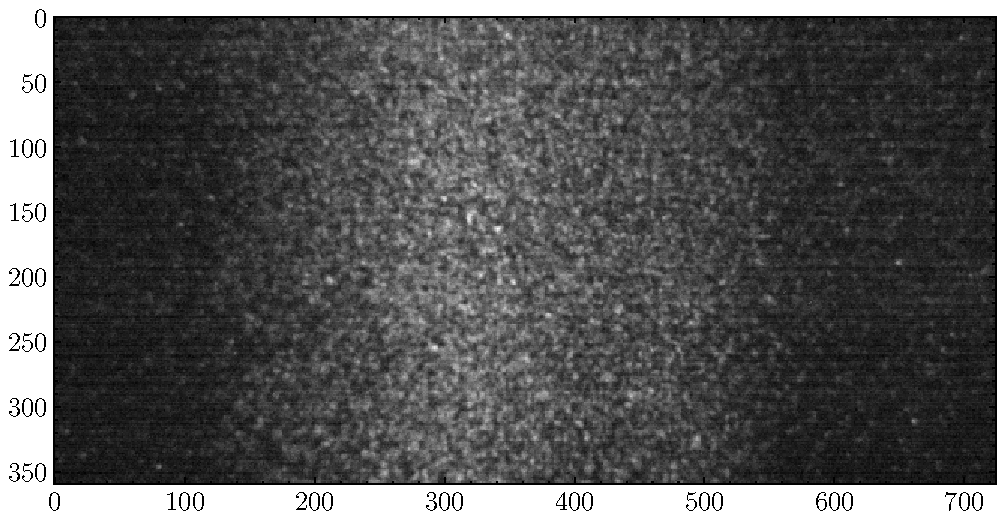
\includegraphics[width=\textwidth]{04_IPHI_Test/figures/fig000_limits_IPHI_a}
    \caption{Beam image}
    \label{chap4:limits_IPHI_a}
  \end{subfigure}

  \begin{subfigure}[t]{1\textwidth}
    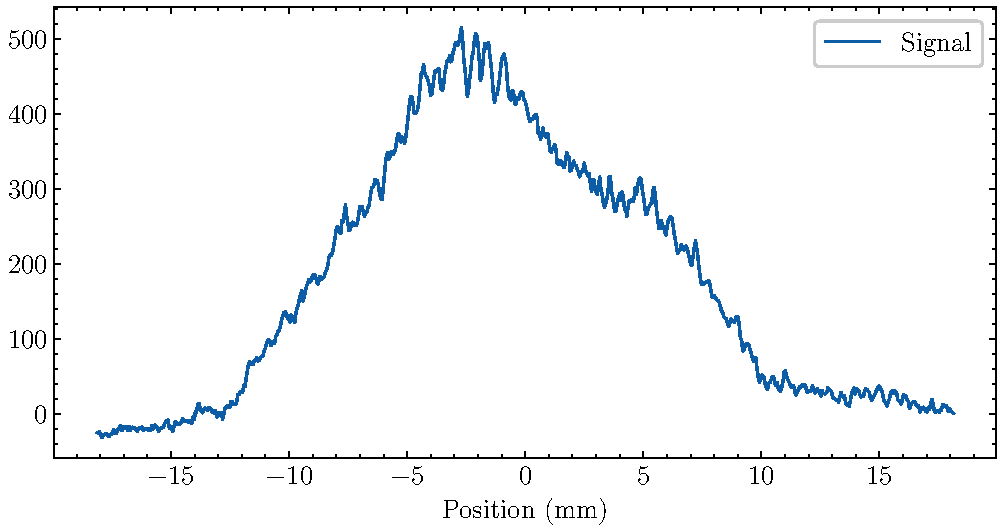
\includegraphics[width=\textwidth]{04_IPHI_Test/figures/fig000_limits_IPHI_b}
    \caption{Projection}
    \label{chap4:limits_IPHI_b}
  \end{subfigure}
  \caption[Example of profile measurement at very low duty cycle.]{Example of profile measurement at very low duty cycle: $0.7\,\mathrm{mA}$, $50\, \mathrm{\mu s}$ and $4 \cdot 10^{-8}\,\mathrm{mbar}$.}
  \label{chap4:limits_IPHI}
\end{figure}


  \subsection{Electron measurement with MCP [C]}
  Unfortunately, we were not able to measure any profile in electron mode during the first and the second campaign.
  Typical pictures in the electron configuration are shown in Figure \ref{chap4:electron_MCP}. One can see that the profiles cannot be measured correctly since an higher signal is observed on the sides of the MCPs. The shapes of noise background look similar.
  The MCPs are in general a little less sensitive to electrons compared to ions at energies between $5$ and $10\,\mathrm{keV}$ \cite{Wiza1979}.
  However, during tests the signals on the camera were always far higher for electrons without any modifications of the gain or the beam conditions.
  Hence, we suppose that the electron background is huge at IPHI.
  During tests, permanent magnets have been installed close to the aperture and beam dump. No clearly improvements have been observed. We still don't know why there is so many electrons.
  \begin{figure}[!ht]
	\begin{subfigure}[t]{0.5\textwidth}
		\includesvg[width=\textwidth]{04_IPHI_Test/figures/fig000_electron_Hamamatsu.svg}
		\caption{Profile measurement attempt with electrons, Hamamatsu MCP.}
		\label{}
	\end{subfigure}
	~
	\begin{subfigure}[t]{0.5\textwidth}
		\includesvg[width=\textwidth]{04_IPHI_Test/figures/fig000_electron_Photonis.svg}
		\caption{Profile measurement attempt with electrons, Photonis MCP.}
		\label{}
	\end{subfigure}
	\caption[Example of images in electron mode]{Example of images in electron mode for both MCPs.
  Some patterns seem to be the same in the edges and middle of the images.
  The line in the middle is not correlated with the beam.}
	\label{chap4:electron_MCP}
\end{figure}


  \section{Summary [C]}
  \label{ch4:Summary}
  This chapter presented all the developments and tests that have been implemented to address the issues raised in Chapter 3, mainly concerning the choice of the most appropriate readout among three readout technologies. The objective was to experimentally prove the proper functioning of the IPM method under conditions close to those of ESS.

  First, the feasibility of silicon detectors was verified on the IRMA ion implanter. The results show that detection is possible with dihydrogen ions of 15 keV. However, as soon as the energy is lower or the ions are heavier, detection is compromised. That is why we have not chosen to continue in this direction.

  The design of the prototypes and the test bench focused on the two remaining methods: strips and MCPs. The IPMs and the test bench have been designed to be very versatile, allowing multiple configurations to be tested. Particular attention was paid to system control and vacuum monitoring. The test bench was installed at IPHI, a 3 MeV proton accelerator, and two test campaigns were carried out.
  % TODO: Commenter plus les résultats

  The first conclusion from the tests shows that the use of a MCP is mandatory to detect signal at ESS conditions. Hence, the optical IPM is the preferred solution since it provides higher sensitivity with respect to the strips alone. A relative check of the electrical field uniformity has been performed on both asymmetric and symmetric configurations and with an optical IPM. The results from the tests show a good agreement with COMSOL simulations.
  Unfortunately, the reference measurements were not exploitable in the experimental conditions but a good agreement between BPMs and IPMs gives more confidence on the measurements.

  We validated our detectors and simulation models as much as experimental condition permitted, in spite of the instability of the machine and not so well-known beam conditions, a rather complete characterization of the prototypes has been achieved.

  From the lessons learned with the prototype, a final design of the cNPM is delivered, including few modifications from the prototype. This will be presented in the concluding chapter.

  \cleardoublepage
  \section{Bibliography}
  \label{ch4:bib}
  \printbibliography[heading=subbibliography]

\end{refsection}
